\graphicspath{{img/capture_baryons/}}
%%%%%%%%%%%%%%%%%%%%%%%%%%%%%%%%%%%%%%%%%%%%%%%%%%%%%%%%%%%%%%%%%%%%%
%%%%%%%%%%%%%%%%%%%%%%%%%%%%%%%%%%%%%%%%%%%%%%%%%%%%%%%%%%%%%%%%%%%%%
%%%%%%%%%%%%%%%%%%%%%%%%%%%%%%%%%%%%%%%%%%%%%%%%%%%%%%%%%%%%%%%%%%%%%
\chapter{Capture on Baryonics in Neutron Stars}
\label{chapter:capture_baryons}

\begin{synopsis}
   This chapter is based on the papers~\cite{Bell:2020obw_sep_NucleonStructureStrong,Anzuini:2021lnv_nov_Improvedtreatmentdark}, where we incorporate two important effects that are important when considering dark matter capture from baryons in neutron stars. 
   % Up to this point, all the results presented have assumed that the DM is scattering off point-like particles that are treated as a free Fermi gas. 
   As the momentum transfers involved in the scattering events leading to capture are large, one must account for the internal structure of the baryon. In addition, the high densities of neutron star matter require us to take into account the strong interactions experienced amongst the baryons. We discuss how to properly incorporate both of these effects into the capture formalism presented in this thesis in a self-consistent manner, and discuss their effects on the capture and interaction rates as well as on the threshold cross-sections that a future NS observation would be sensitive to. 
\end{synopsis}
%%%%%%%%%%%%%%%%%%%%%%%%%%%%%%%%%%%%%%%%%%%%%%%%%%%%%%%%%%%%%%%%%%%%%
%%%%%%%%%%%%%%%%%%%%%%%%%%%%%%%%%%%%%%%%%%%%%%%%%%%%%%%%%%%%%%%%%%%%%
%%%%%%%%%%%%%%%%%%%%%%%%%%%%%%%%%%%%%%%%%%%%%%%%%%%%%%%%%%%%%%%%%%%%%

%%%%%%%%%%%%%%%%%%%%%%%%%%%%%%%%%%%%%%%%%%%%%%%%%%%%%%%%%%%%%%%%%%%%%
%%%%%%%%%%%%%%%%%%%%%%%%%%%%%%%%%%%%%%%%%%%%%%%%%%%%%%%%%%%%%%%%%%%%%
\section{Baryon Structure and Strong Interactions}
\label{ch5:sec:baryons_in_NSs}
%%%%%%%%%%%%%%%%%%%%%%%%%%%%%%%%%%%%%%%%%%%%%%%%%%%%%%%%%%%%%%%%%%%%%
%%%%%%%%%%%%%%%%%%%%%%%%%%%%%%%%%%%%%%%%%%%%%%%%%%%%%%%%%%%%%%%%%%%%%

%%%%%%%%%%%%%%%%%%%%%%%%%%%%%%%%%%%%%%%%%%%%%%%%%%%%%%%%%%%%%%%%%%%%%
\subsection{Baryon Effective Masses}
\label{ch5:subsec:strong_ints_meffs}
%%%%%%%%%%%%%%%%%%%%%%%%%%%%%%%%%%%%%%%%%%%%%%%%%%%%%%%%%%%%%%%%%%%%%

At the extremely high densities found in the interiors of neutron stars, the strong interactions amongst the baryons render the free Fermi gas approximation used in Chapter~\ref{chapter:capture_intro} to model the scattering targets invalid. To account for these interactions in a self-consistent way, they should be included in the Lagrangian used to model the nucleon-rich matter. This is often achieved by including effective Skyrme forces, or through a relativistic mean field theory.

The QMC EoS, described in Section~\ref{ch2:subsec:NS_EoS}, adopts the latter approach. The forces mediated by the Lorentz scalars induce an effective mass for the baryons different from their vacuum value, such that $\mbeff \leq \mi$. In this model, the single particle energy for a baryon with momentum $\vec{p}_i$ can be expressed as
\begin{equation}
   \Ei(p_i) = \sqrt{p_i^2 + [\mbeff(n_b)]^2} + U_i(n_b),
   \label{ch5:eq:total_energy}
\end{equation}
where $U_i(n_b)$ is the potential induced by the Lorentz vector forces, which depends on the baryon number density. This expression resembles the dispersion relation for a particle of mass $\mbeff$ under the influence of an external force with corresponding potential $U_i$. Hence, the single-particle energy spectrum of the interacting baryons must be expressed in terms of $\mbeff$ rather than the mass in vacuum, and it is this mass that will enter into the kinematics of the scattering processes.  

Accounting for the strong interactions in this way leads to several modifications to the results obtained in Chapter~\ref{chapter:capture_intro}. Firstly, all appearances of the bare mass $\mi$ are replaced by $\mbeff$ in all the results. This will lead to non-trivial modifications of the capture and interaction rates throughout the star as the mass of the target will decrease deeper into the star (see right panels of Fig.~\ref{ch2:fig:QMC_profiles}).

In addition, the Fermi energies, $\kinFi = \muFi - \mi$, are now calculated according to 
\begin{equation}
   \kinFi(r) = \sqrt{[p_{F,i}(n_i)]^2 + [\mbeff(r)]^2} - \mbeff(r),
   \label{ch5:eq:kinFe_meff}
\end{equation}
where $p_{F,i}$ is the Fermi momentum of species $i$. This becomes the input to the Fermi-Dirac distributions for the capture and interaction rates. In doing this, the number density evaluated in the free Fermi gas apprioximation, Eq.~\ref{ch3:eq:n_free_Fermi}, becomes equal to the true number density, $n_i(r)$, provided by solving the EoS alongside the TOV equations. To see this, substitute Eq.~\ref{ch5:eq:kinFe_meff} into Eq.~\ref{ch3:eq:n_free_Fermi} and make the replacement $\mi\rightarrow \mbeff$ to gets
\begin{align}
   n_\mathrm{free}(\kinFi(r), \mbeff(r)) & = \frac{1}{3\pi^2}\left[ \kinFi(r)(2\mbeff + \kinFi(r))\right]^{3/2}\\
   & = \frac{(p_{F,i}(r)^2 + [\mbeff]^2)^{3/2}}{3\pi^2}\\
   & = \frac{p_{F, i}^3}{3\pi^2}\\
   & = n_i(r)
\end{align}
for a Fermi gas, interacting or otherwise. 
As such, the correction factor used to correct for usign realistic profiles for the target is now $\zeta(r) = 1$.


%%%%%%%%%%%%%%%%%%%%%%%%%%%%%%%%%%
\begin{figure}[t!bp]
   \centering
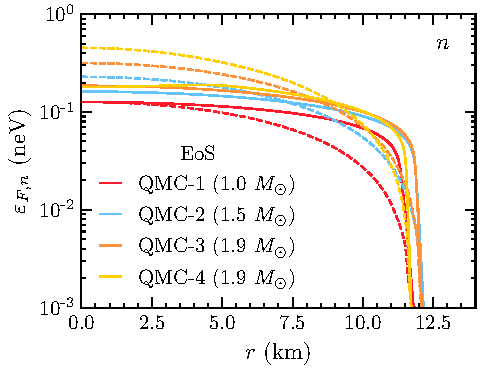
\includegraphics[width=0.495\textwidth]{capture_3/muFn_meff_r_QMC.pdf}
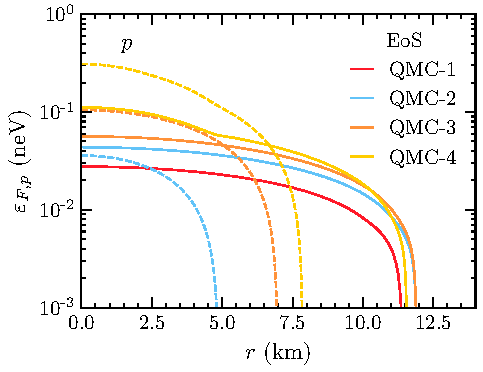
\includegraphics[width=0.495\textwidth]{capture_3/muFp_meff_r_QMC.pdf}
   \caption{Radial profiles of the Fermi energy for neutrons (left) and protons (right). Results are shown for the free Fermi gas (dashed) and interacting baryon (solid) approaches, for the benchmark NS configurations of Table~\ref{ch2:tab:QMC_configs}.
   }
   \label{ch5:fig:muradprofs}
\end{figure}
%%%%%%%%%%%%%%%%%%%%%%%%%%%%%%%%%

In Fig.~\ref{ch5:fig:muradprofs} we show the values of the Fermi energies for neutrons (left panel) and protons (right panel). The dashed lines are the radial profiles used in the free Fermi gas approximation and the solid lines correspond to the calculation outlined above for the effective mass approach. We immediately notice that the profiles for the free Fermi gas approximation are steeper, having larger values in the core and decreasing more rapidly towards the surface, while those obtained with the effective mass approach are quite flat, especially in the core, and go to zero only very close to the surface.

The difference between these two calculations is significantly more prominent for protons. Specifically, in the free Fermi gas approach, we find that protons are non-degenerate in the outer regions of the core and, for light NS configurations such as QMC-1, are non-degenerate throughout the whole star.\footnote{Not shown in Fig.~\ref{ch5:fig:muradprofs} because of the logarithmic scale.}
In contrast, protons are degenerate throughout the entire star in the interacting baryon treatment. 
As we shall see, these different Fermi energies will have important consequences when calculating DM capture and interaction rates, especially for proton targets.


%%%%%%%%%%%%%%%%%%%%%%%%%%%%%%%%%%%%%%%%%%%%%%%%%%%%%%%%%%%%%%%%%%%%%
\subsection{Momentum Dependence of Hadronic Form Factors}
\label{ch5:subsec:mom_dep_FF}
%%%%%%%%%%%%%%%%%%%%%%%%%%%%%%%%%%%%%%%%%%%%%%%%%%%%%%%%%%%%%%%%%%%%%

In the preceding chapters, we had regarded the target as a point-like particle that the DM scattered off, which is perfectly valid for the leptonic species. Baryons, on the other hand, are composite particles made of three valence quarks and hence have a finite size. When the momentum transfer exceeds the inverse Compton wavelength of the baryon, $\sim 1/\lambda_\mathcal{B} \sim m_\mathcal{B}$, the internal strucyre begins to be probed, and we must account for their finite size.

As discussed in Section.~\ref{ch1:subsec:quark_to_nucleon_EFT}, this is achieved by reintroducing the momentum dependence in the hadronic form factors, 
\begin{align}
   c_\mathcal{B}^I(t)  &= c_\mathcal{B}^{I}(0) F^2(t),\quad I\in\{S, P, V, A, T\},\\
   F(t) & = \frac{1}{(1 - t/Q_0^2)^2},\label{ch5:eq:FF_def}
\end{align}
where $t$ is the Mandelstam variable, $Q_0$ is an energy scale taken to be $0.9\GeV$, and $c_\mathcal{B}^I(0)$ are the form factors evaluated at zero momentum transfer, with their values given in Appendix~\ref{app:hadronic_matrix_elements}. This factor is included in the matrix elements of the operators in Table.~\ref{ch1:tab:opers_defn_full}, and as such modifies the analytic result for the interaction rate derived in Section~\ref{ch3:sec:diff_int_rate} for matrix elements $\Msq \propto t^n s^m$ to become
\begin{equation}
   \begin{split}
       \Gamma^{-}(E_\chi) & \propto \frac{(-1)^n }{128\pi^3 E_\chi k }\int_0^{E_\chi -m_\chi} dq_0\int \, dt_E \frac{ t_E^n}{(t_E + q_0^2)^{m+\frac{1}{2}}}\frac{1}{(1 + t_E/Q_0^2)^4}\\
       &\hspace{4em}\times\sum_{r=0}^m \mathcal{V}_{m,r}\sum_{j = 0}^r\binom{r}{j} \kinFi^{r-j}  \frac{(-1)^{j} q_0^{j+1}}{j+1} h_j\left( \frac{\Ei^{t^-} - \kinFi}{q_0}\right),
   \end{split}
   \label{ch5:eq:gammaFFfinaltext}
\end{equation}
where $E_i^{t^-}$ and $h_j(x)$ are given in Eqs.~\ref{ch3:eq:Etm_def} and~\ref{ch3:eq:h_stepfn} respectively.

The main effect of these form factors is the suppression of high momentum transfer interactions. This will also increase the DM mass range over which Pauli blocking is expected to be active. We can see these effects by examining the kinematically allowed regions of phase space together with the differential interaction rate profiles.


%%%%%%%%%%%%%%%%%%%%%%%%%%%%%%%%%%%%
\begin{figure}[t!bp] 
   \centering
   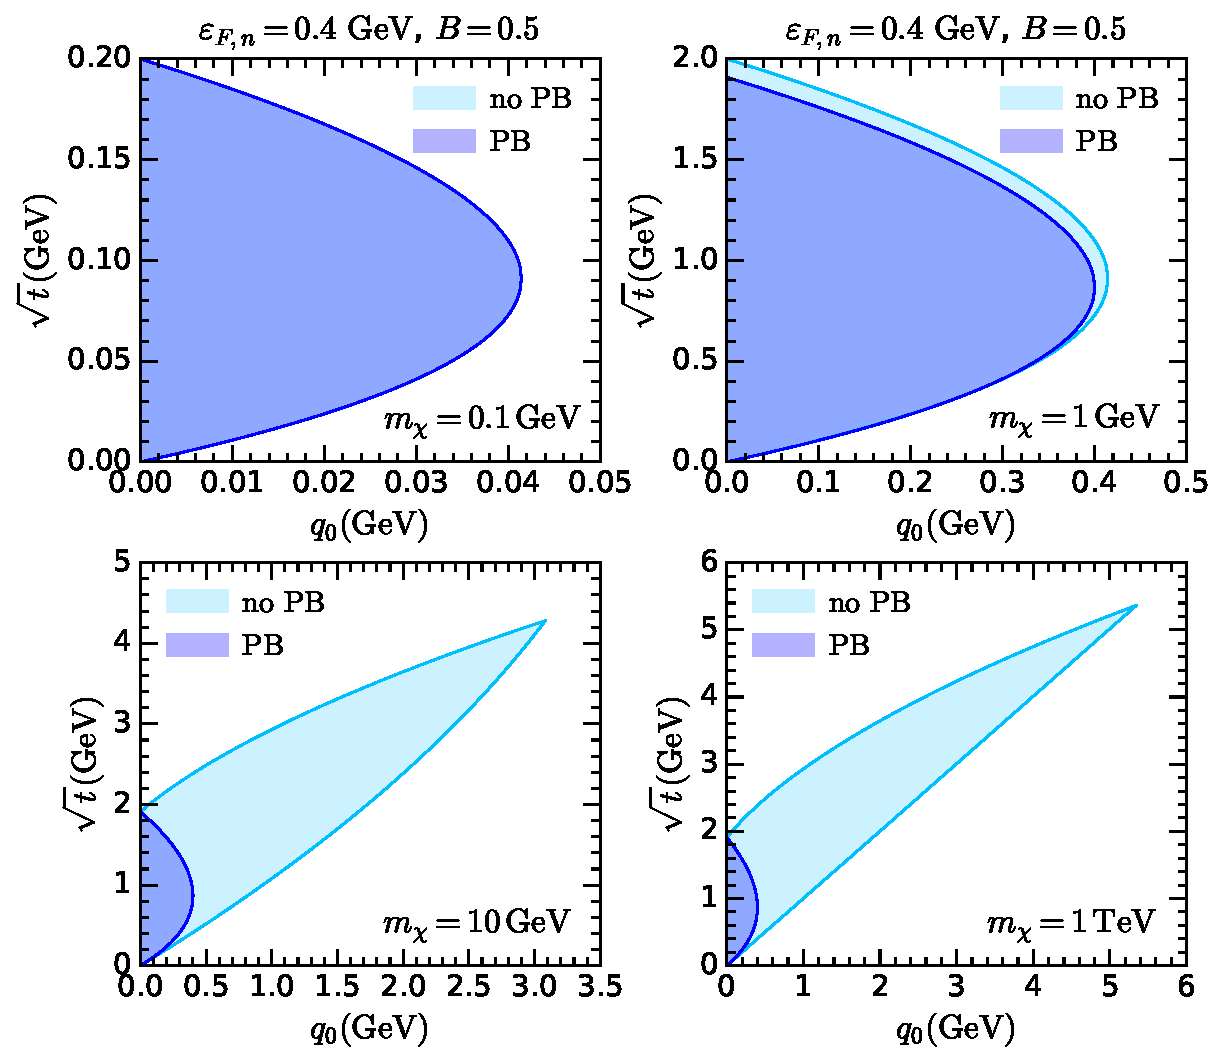
\includegraphics[width=0.75\textwidth]{capture_3/C_int_domain_mdm.pdf}
   \caption{Integration domain for the interaction rate, for different choices of DM mass, assuming   
     $B=0.5$ and $\kinFn=0.4\GeV$. The kinematically allowed region is shaded in light blue and the Pauli suppressed region (PB) in dark blue. 
   }
   \label{ch5:fig:intC}
   \end{figure}
   %%%%%%%%%%%%%%%%%%%%%%%%%%%%%%%%%%%%
   
   
In Fig.~\ref{ch5:fig:intC}, we show how Pauli blocking affects the integration domain of Eq.~\ref{ch5:eq:gammaFFfinaltext}, which is controlled by the smoothed step function $h_0(x)$, for some representative choices of DM mass and the benchmark values $\kinFn=0.4\GeV$ and $B=0.5$.  The region where $h_0(x)=0$ is not kinematically allowed and hence not shown in Fig.~\ref{ch5:fig:intC}.
The light blue area represents the region that is not affected by Pauli blocking (PB), i.e. $h_0(x)=-x$, while the dark blue shaded area indicates the PB region, where $h_0(x)=1$. 
We observe that for light DM masses such as  $m_\chi=0.1\GeV$ (top left panel), the whole domain lies in the PB region. For $m_\chi=1\GeV$ (top right panel), there is a tiny slice of the domain that is not Pauli suppressed. The picture changes dramatically when the DM mass is increased to $m_\chi=10\GeV$ (bottom left panel), where almost the whole integration domain is unaffected by PB. Increasing the DM mass even further, e.g., up to $m_\chi=1\TeV$ (bottom right panel) does not result in much further change to the shape of the domain, demonstrating that the transition between the PB and non-PB regimes occurs between $m_\chi\sim1\GeV$ and $m_\chi\sim10\GeV$.
   


%%%%%%%%%%%%%%%%%%%%%%%%%%%%%%%%%%%%%%%%%%%
\begin{figure}[t!bp] 
\centering
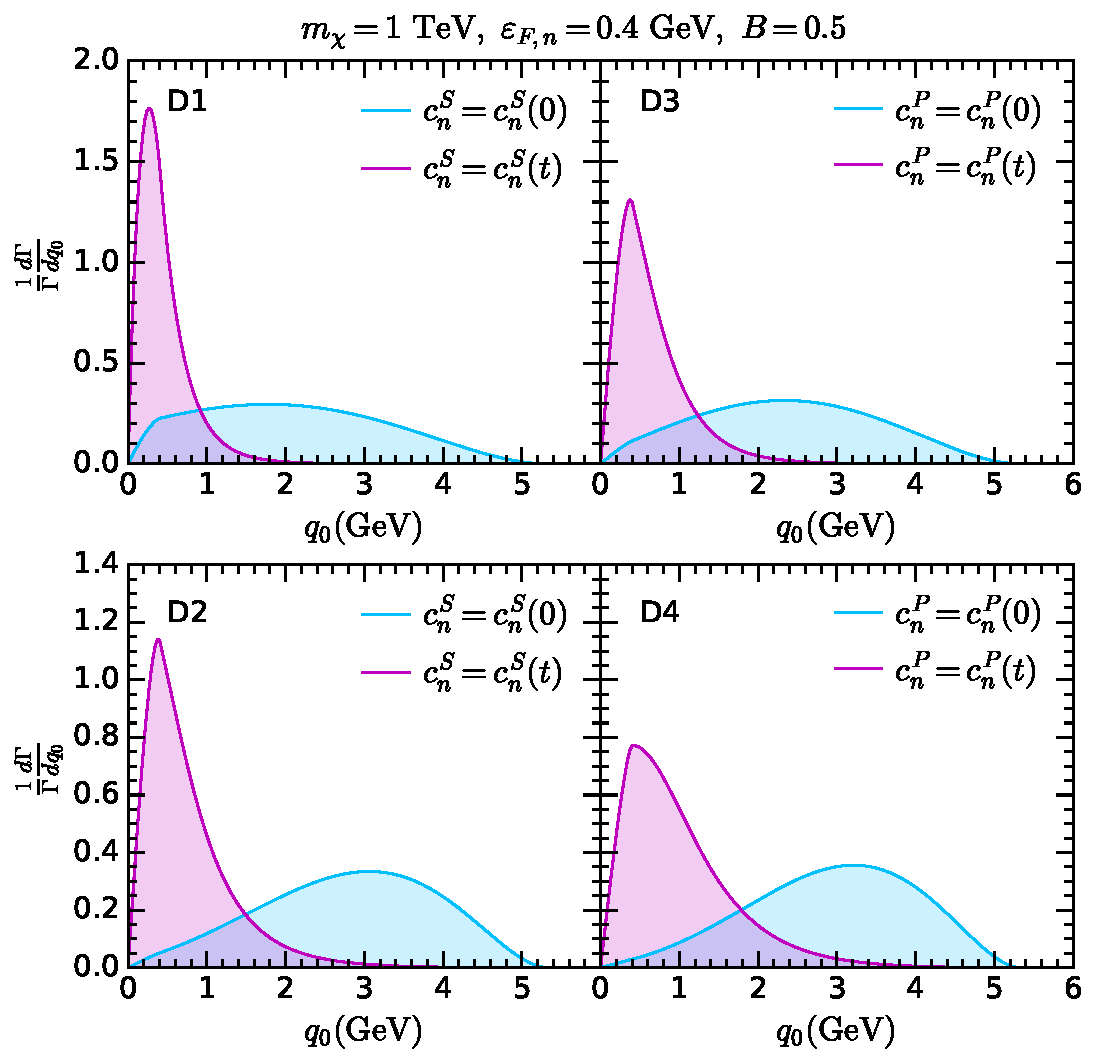
\includegraphics[width=0.95\textwidth]{capture_3/norm_diff_intrate_q_D1-D4.pdf} 
\caption{Normalised differential DM-neutron interaction rate as a function of the DM energy loss, $q_0$, for the operators D1 (top left), D3 (top right), D2 (bottom left) and D4 (bottom right). The light blue lines denote the interaction rate calculated using constant neutron form factors $c_n^S(0)$, $c_n^P(0)$, while the orange lines correspond to that for momentum-dependent couplings $c_n^S(t)$, $c_n^P(t)$. We have set $m_\chi=1\TeV$, $B=0.5$, $\kinFn=0.4\GeV$.
}
\label{ch5:fig:intrateqtr1}
\end{figure}
%%%%%%%%%%%%%%%%%%%%%%%%%%%%%%%%%%%%%%%%%%%



In Fig.~\ref{ch5:fig:intrateqtr1} we show the normalised differential interaction rates for operators D1-D4 as a function of the energy loss $q_0$, calculated with (orange) and without (light blue) momentum dependent couplings, for neutron targets and $m_\chi=1\TeV$. In all cases, we observe that the inclusion of $t$-dependent hadronic matrix elements shifts the peak of the spectrum towards lower energy transfers, $q_0$. 
Thus, the inclusion of $c_i^I(t)$ in Eq.~\ref{ch5:eq:gammaFFfinaltext} suppresses DM-neutron interactions at large momentum transfers. 
Replacing the target mass with the corresponding effective mass $\mbeff\leq m_i$ also shifts the average energy transfer to lower energies.  When both effects are present, a lighter target mass reduces the suppression arising from $t$-dependent form factors. 

%%%%%%%%%%%%%%%%%%%%%%%%%%%%%%%%%%%%%%%%%%%%%%%%%%%%%%%%%%%%%%%%%%%%%
\subsubsection{Asside: Deep Inelastic Scattering}
\label{ch5:subsubsec:DIS}
%%%%%%%%%%%%%%%%%%%%%%%%%%%%%%%%%%%%%%%%%%%%%%%%%%%%%%%%%%%%%%%%%%%%%
Given that the momentum transfer in the DM-nucleon scattering process is sufficiently large that we cannot treat the nucleons as point particles (up to $\sim 10\GeV$ in the cores of the heaviest NSs), one may wonder if there are sizable contributions from Deep Inelastic Scattering (DIS). To that end, we examine the contribution from DIS to the total DM-neutron scattering cross-section. 

The kinematics of DIS of dark matter in NSs is not similar to any case that has previously been treated in the literature, at least not to our knowledge. In contrast to DIS of neutrinos and boosted DM, we are interested in much larger DM masses and relatively lower energies.  Specifically, $E_\chi/m_\chi=1/\sqrt{B}$, where $B$ is the time component of the Schwarzchild metric, which falls in the range $[\sim0.2,\sim0.75]$.  Therefore, we have  $E_\chi\lesssim 2m_\chi$. Following ref.~\cite{Agashe:2014yua_Directdetectionboosted}, we derive the DIS cross-section in NSs for the operators in Table~\ref{ch1:tab:opers_defn_full}. 

The parton level differential cross-section is given by
\begin{equation}
    \frac{d\hat{\sigma}}{d\hat{t}} = \frac{\hat{s}}{8\pi\hat{\gamma}^2}\frac{\hat{s}-(m_\chi^2+x^2m_n^2)}{\hat{s}^2-(m_\chi^2-x^2m_n^2)^2}|\overline{\mathcal{M}}(\hat{s},\hat{t},m_i=x m_n)|^2,
\end{equation}
where $\hat{\gamma} = \gamma(\hat{s}, m_\chi, xm_n)$, $\hat{t}=-Q^2$ is the squared 4-momentum transfer,  $\hat{s} = (1-x)(m_\chi^2-x m_n^2) +xs$, $\Msq$ is defined at the parton level with couplings $g_i=g_q$, and $x$ is the fraction of the nucleon momentum ($P$) carried by the parton, $p=xP$. We define $y$, the fractional energy lost by the DM in the nucleon rest frame~\cite{Agashe:2014yua_Directdetectionboosted}
\begin{equation}
    y = \frac{2q\cdot P}{2k\cdot P} = \frac{-\hat{t}}{\hat{s}-m_\chi^2-x^2m_n^2}, 
\end{equation}
and obtain
\begin{equation}
    dQ^2 = (\hat{s}-m_\chi^2 - x^2m_n^2)dy = x(s - m_\chi^2 - m_n^2)dy. 
\end{equation}
We then use the parton distribution functions (PDFs), $f_i$, to obtain the nucleon level differential DIS cross-section
\small
\begin{equation}
    \frac{d^2\sigma}{dx\, dy} =(\hat{s} - m_\chi^2-x^2m_n^2) \frac{\hat{s}}{8\pi\hat{\gamma}^2}\frac{\hat{s}-(m_\chi^2+x^2m_n^2)}{\hat{s}^2-(m_\chi^2-x^2m_n^2)^2}\sum_i f_i(x, Q^2)|\overline{\mathcal{M}}(\hat{s},\hat{t},x m_n)|^2.
\end{equation}
\normalsize
The integration bounds for the DIS cross-section are generically $0<x<1$ and $0<y<y_{max}$, where $y_{max}$ is set by imposing $\cos\theta\leq 1$, and in general $y_{max}\neq 1$~\cite{Agashe:2014yua_Directdetectionboosted}.  The value of $y_{max}$ is set by
\begin{equation}
    y_{max} = \frac{-\hat{t}_{min}}{\hat{s} - m_\chi^2 - x^2 m_n^2}
     = \frac{(\hat{s} -m_\chi^2 -x^2m_n^2)^2 - 4 x^2 m_\chi^2 m_n^2}{\hat{s}(\hat{s} -m_\chi^2 - x^2m_n^2)}. 
\end{equation}

The capture rate requires integrating the differential cross-section over $\hat{s}$, which must be done at the parton level, i.e., before integrating over $x$. We perform this integration over the centre of mass energy by following the same procedure performed for capture in the intermediate mass regime outlined in Section.~\ref{ch3:subsec:captureintermediate}. The differential capture rate will then scale as 
\begin{align}
   \frac{dC}{dr}\propto \int_0^1 dx\int_{\hat{s}_0-\delta\hat{s}}^{\hat{s}_0+\delta\hat{s}}d\hat{s}\int_0^{y_{max}}dy  \frac{d^2\sigma}{dx\, dy} \,\Theta(Q^2 -1\GeV^2), \label{eq:DIS}
\end{align}
where the step function enforces the momentum transfer to be above the $1\GeV$ threshold where the PDFs are reliable, and 
\begin{align}
    \hat{s}_0 & = m_\chi^2 + 2x E_n E_\chi,\\
    \delta\hat{s} & = 2xm_\chi \sqrt{E_n^2 -m_n^2}\sqrt{\frac{1-B(r)}{B(r)}},\\
    E_n & \simeq m_n + \mu_{F,n}. 
\end{align}
We numerically evaluate the DIS cross-section using the MSTW2008 NLO PDFs~\cite{Martin:2009iq_PartondistributionsLHC}. 

In Fig.~\ref{ch5:fig:DISratio}, we show the ratios of the elastic (EL) and deep inelastic scattering (DIS) cross-sections
to the total cross-section (TOT=DIS+EL),  as a function of the radial coordinate $r$ for the NS  QMC-4, neutron targets and $m_\chi=10^6\GeV$. We consider two scenarios: the free Fermi gas approach and the interactive baryon approach characterised by $\mneff$. The radial coordinate determines the value of $B$, the Fermi energy of the target, and $\mneff$. 

In both the $\mneff$ and free Fermi gas approaches, the DIS contribution (light blue and green lines, respectively) increases towards the centre of the star, where $B$ takes lower values and hence the DM kinetic energy is higher. The ratio $\sigma^{DIS}/\sigma^{TOT}$ is smaller in the $\mneff$ approach, compared to the free Fermi gas approach, due to a smaller neutron effective mass. In the correct interactive baryon approach, the ratio of the DIS contribution (light blue lines) to the total cross-section is at most ${\cal O}(40\%)$ at the centre of the star for D8, ${\cal O}(20\%)$ for D7, D9-D10, and much lower for the remaining operators.  

As a result, for most operators, the elastic cross-section provides a very good approximation to the total cross-section (compare magenta with dashed blue lines).
Note that these cross-sections are weighted by $r^2dr$ in the capture rate calculation of Eq.~\ref{ch3:eq:cap_rel_full_1} (i.e. weighted by volume) which further reduces the importance of the DIS contribution. 

It is worth noting that we have neglected the effect of Pauli blocking on the DIS cross-section. In deep inelastic scattering, one must have a baryon in the final state and with a nucleon target this is almost always a nucleon. As shown in both theoretical calculations~\cite{Melnitchouk:1992gd_Protonproductionbias} and direct experimental studies~\cite{BEBCWA59:1989ayi_Backwardparticleproduction}, this nucleon has low momentum in the laboratory frame, typically 300 MeV or less. Such nucleons will be totally Pauli blocked in the core of a NS, and hence the deep inelastic cross-section drastically reduced. 
As a result, the contribution of the deep inelastic process to the capture rate will have a negligible effect on our conclusions. 

We performed a similar calculation for hyperon targets and found that as for neutrons, the DIS contribution to the total cross-section is more important for operators D7-D10 in the absence of Pauli blocking of the fragmented baryonic final states. For D8 and  $\Xi^-$ targets, the DIS cross-section can even surpass the elastic scattering contribution (including form factors) and reach $\sim60\%$ of the total cross-section at the centre of the star.  $\Xi^-$ provides the largest hyperonic contribution to the capture rate, however, this (elastic scattering) contribution is already more than one order of magnitude lower than that of neutrons for D7-D10.  
Even if Pauli blocking does not suppress the DIS final states, the contribution of the deep inelastic process to the capture of DM is negligible, since it would enhance the capture rate by scattering on $\Xi^-$ at most by a factor of $\sim2$. 

\begin{figure}[t!bp]
    \centering
    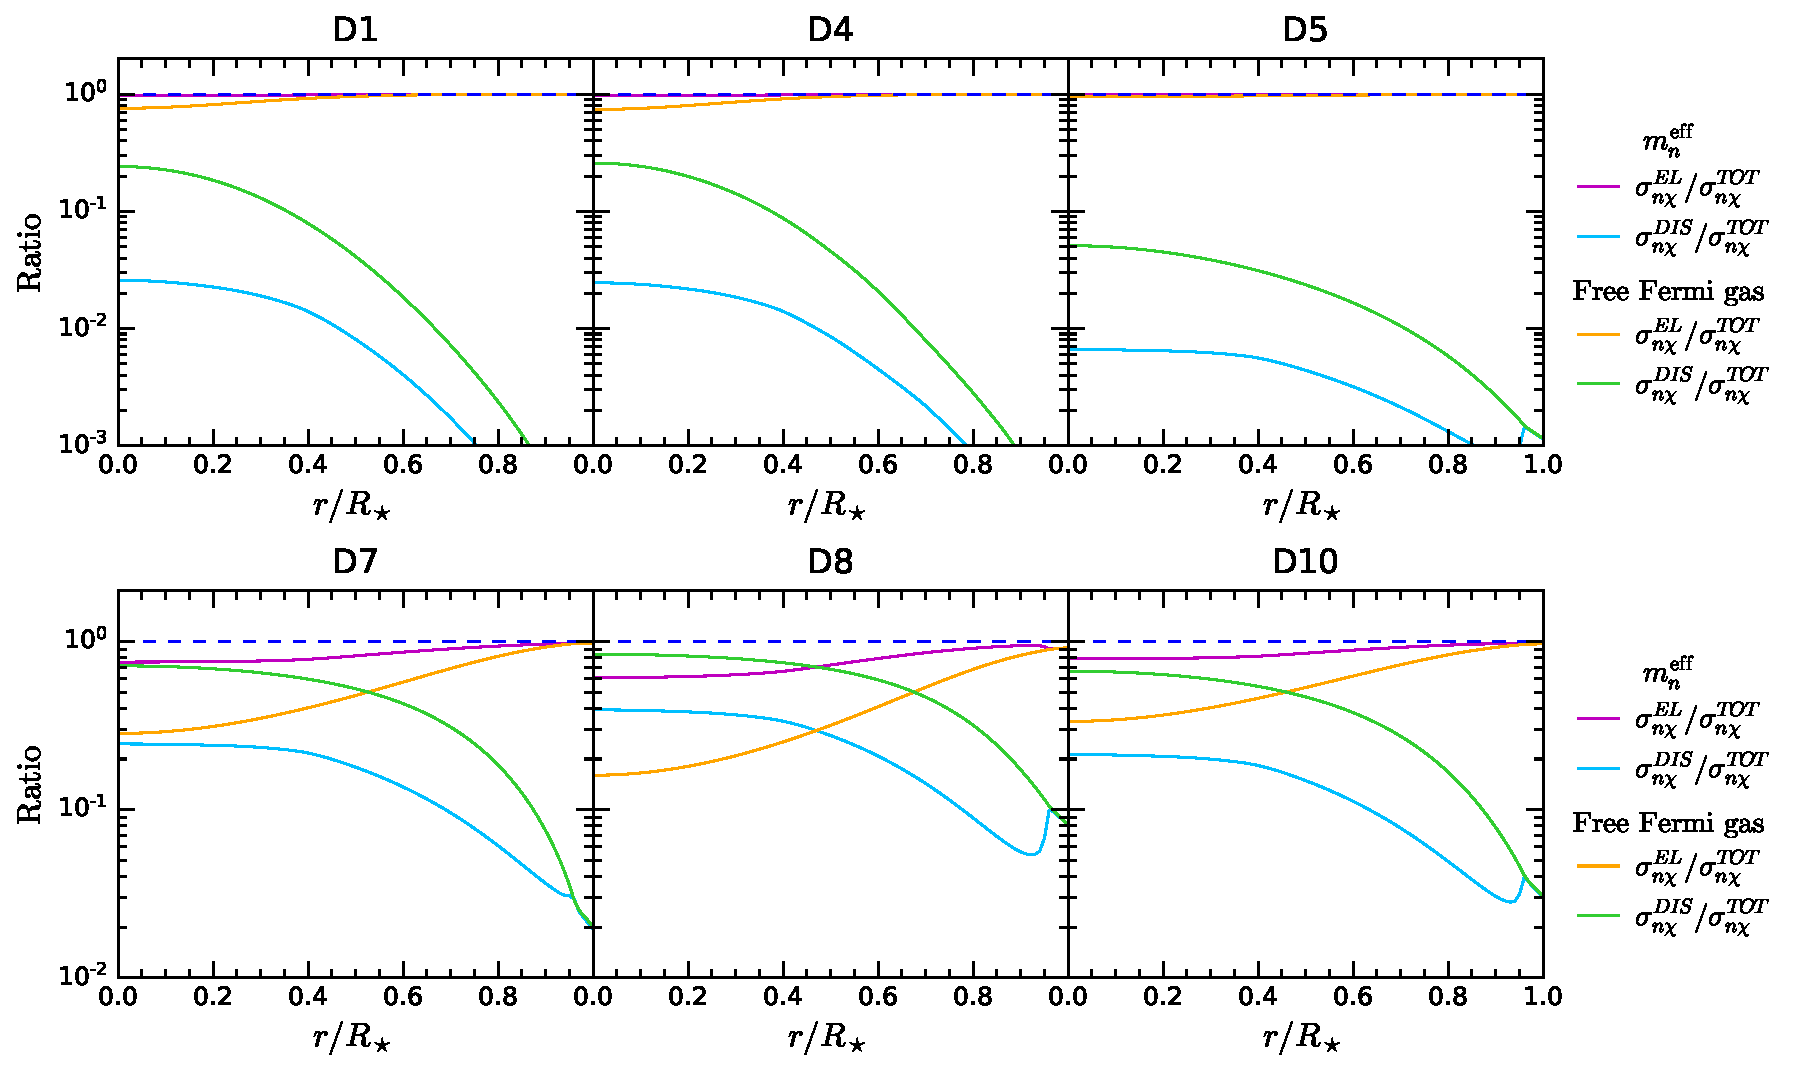
\includegraphics[width=\textwidth]{capture_3/DIS_xsectot_ratio_PeV.pdf}
    \caption{Ratios of the elastic (EL) and deep inelastic scattering (DIS) cross-sections to the total cross-section (TOT=EL+DIS) as a function of the NS radius, for neutron targets in the NS QMC-4 and six of the dimension-6 EFT operators.  We have taken $m_\chi=10^6\GeV$, and shown the comparison for both the interacting baryon and free Fermi gas approaches. Momentum-dependent form factors have been included in the elastic calculations.  }  
    \label{ch5:fig:DISratio}
\end{figure}

In addition to DIS, there may, in principle, be a contribution from the excitation of baryon resonances.  However, the resonance excitation cross-section is also expected to be suppressed. In NSs, the mass of the $\Delta$ baryon, which gives the largest contribution to this cross-section, increases with the baryon number density by between $\sim100$ and $300 \MeV$~\cite{Motta:2019ywl_Deltabaryonsplay}. This will suppress the resonance excitation cross-section significantly. Therefore, we consider only elastic collisions. 


%%%%%%%%%%%%%%%%%%%%%%%%%%%%%%%%%%%%%%%%%%%%%%%%%%%%%%%%%%%%%%%%%%%%%
%%%%%%%%%%%%%%%%%%%%%%%%%%%%%%%%%%%%%%%%%%%%%%%%%%%%%%%%%%%%%%%%%%%%%
\subsection{Modifications to the Capture Rate}
\label{ch5:subsection:capture_modification}
%%%%%%%%%%%%%%%%%%%%%%%%%%%%%%%%%%%%%%%%%%%%%%%%%%%%%%%%%%%%%%%%%%%%%
%%%%%%%%%%%%%%%%%%%%%%%%%%%%%%%%%%%%%%%%%%%%%%%%%%%%%%%%%%%%%%%%%%%%%
\subsubsection{Low and Intermediate Mass Regime}
We now incorporate the effects discussed above into the expressions for the capture rates derived in Chapter~\ref{chapter:capture_intro}. In the low mass regime, where Pauli blocking is relevant, the modifications are minor, and we simply replace $\mi\rightarrow \mbeff$ in Eqs.~\ref{ch3:eq:cap_rel_full_1} and~\ref{ch3:eq:int_rate_capture_full} and set $\zeta(r) = 1$, as the form factors are incorporated in the matrix elements. We write these explicitly here for clarity,
% 
\begin{align}
   C & =\frac{4\pi}{v_\star}\frac{\rho_\chi}{m_\chi} \erf\left(\sqrt{\frac{3}{2}}\frac{v_\star}{v_d}\right) \int_0^{R_\star}  r^2\frac{\sqrt{1 - B(r)}}{B(r)}\Omega^-(r)\,dr,
   \label{ch5:eq:cap_general}\\
   \begin{split}
      \Omega^-(r) & = \frac{1}{32\pi^3}\int dt\,d\Ei\,ds \frac{|\overline{\mathcal{M}}(s, t, \mbeff)|^2}{\beta(s, \mbeff)\gamma(s, \mbeff)}\frac{\Ei s}{m_\chi}\sqrt{\frac{B(r)}{1 - B(r)}}\\
      &\hspace{14em} \times \fFD(\Ei, r)\left( 1 - \fFD(\Ei', r)\right),
   \end{split}
   \label{ch5:eq:omega_meff_low}
\end{align}
where we have made the $\mbeff$ dependence of the $\beta$ and $\gamma$ functions of Eqs.~\ref{ch3:eq:beta_func} and~\ref{ch3:eq:gamma_func} explicit. 

In the intermediate mass range, where Pauli blocking no longer suppresses the capture rate, we derived the simplified expression Eq.~\ref{ch3:eq:csimplelargemtext_sdep} valid for matrix elements of the form $\Msq \propto \bar{g}(s) t^n$, with $\bar{g}(s)$ some function of the centre of the mass energy, and $n = 0, 1, 2$. While including the effective masses is simple, the inclusion of the momentum-dependent form factors, Eq.~\ref{ch5:eq:FF_def}, complicates the integration over the momentum transfer $t$. Fortunately, we can still write down an analytic expression for the capture rate in this regime, for matrix elements $\Msq \propto \bar{g}(s) t^n F^2(t)$, this being
\begin{equation}
   \begin{split}
      C_\mathrm{appox.} &= \frac{1}{\vstar} \frac{\rho_\chi}{\mchi}\erf\left(\sqrt{\frac{3}{2}}\frac{\vstar}{v_d}\right)\int_0^{\Rstar}dr\,r^2n_i^2(r) \frac{\bar{g}(s_0)}{n+1}\left[2 \mbeff\right]^{2n} \\
      & \hspace{14em}\times\left[\frac{1 - B(r)}{B(r)}\right]^{n+1} \mathcal{F}_n(|t_\mathrm{min}|),
   \end{split}
   \label{ch5:eq:capture_simple}
\end{equation}
with $s_0$ given in Eq.~\ref{ch3:eq:s0}, and the functions $\mathcal{F}_n(|t_\mathrm{min}|)$ are given by
\begin{align}
   \mathcal{F}_n(x) & = \frac{\int_0^x dt\,t^n F^2(t)}{\int_0^x dt\,t^n},\\
   \mathcal{F}_0(x) & = \frac{Q_0^2}{x + Q_0^2},\\
   \mathcal{F}_1(x) & = 2\frac{Q_0^2}{x^2} \left[\log\left(1 + \frac{x}{Q_0^2}\right) - \frac{x}{x + Q_0^2 }\right],\\
   \mathcal{F}_2(x) & = 6 \frac{Q_0^3}{x^3}\left[ -\log\left(1 + \frac{x}{Q_0^2}\right) + \frac{x (x + 2Q_0^2)}{2 Q_0(x + Q_0^2)} ,\right]\\
   |t_\mathrm{min}| & = \frac{\gamma^2(s, \mbeff)}{s} \approx\frac{4 \mchi^2( 1 - B(r))}{B(r)(1 + \mu^2) + 2 \mu\sqrt{B(r)}}.
\end{align}
Note that the $\mathcal{F}_n$ are decreasing functions fo both $n$ and $|t_\mathrm{min}|$, and hence are decreasing functions of the target mass.

\subsubsection{Large Mass Regime}


As discussed in Section~\ref{ch3:subsec:largemassandsigma}, the probability that a DM particle with a mass greater than the threshold value $\mstar$ loses enough energy in a single scatter such that it becomes captured becomes less than 1. The precise value of $\mstar$ depends both on the species the DM scatters with, and the nature of this interaction.  
This reduced capture probability is accounted for by including the factor $c_1(r)$, Eq.~\ref{ch3:eq:c1}, in the expression for the capture rate Eq.~\ref{ch5:eq:capture_simple} for $\mchi\gg m_i$. 

Note that $c_1$ depends on $\kinFi(r)$, $B(r)$ and $m_i$ through the interaction rate $\Gamma^-$.
Aside from $B$, $\mstar$ depends only on 2 quantities that have dimension of energy: the mass of the target $m_i$ and its Fermi energy $\kinFi$. 
Interestingly, if one rescales both $m_i$ and $\kinFi$ by the same factor, the resulting $\mstar$ will just acquire this factor. 
This means that for baryon couplings at zero momentum transfer, we can calculate $\mstar$ for a generic target mass $\mbeff$ by rescaling the values obtained in the free Fermi gas approximation in the following way: 
\begin{equation}
\mstar(\mbeff, \kinFi)= \frac{\mbeff}{m_i} \mstar(m_i,\kinFi\frac{m_i}{\mbeff}).
\end{equation}
However, when including the dependence of the baryon couplings on the transferred momentum an additional energy scale comes into play, namely $Q_0$. Unfortunately, it is not possible to rescale the $\mstar$ values obtained with $c_i^I(0)$ to obtain the correct value required when using $c_i^I(t)$.




%%%%%%%%%%%%%%%%%%%%%%%%%%%%%%%%%%%%%
  \begin{figure}[t!bp]
    \centering
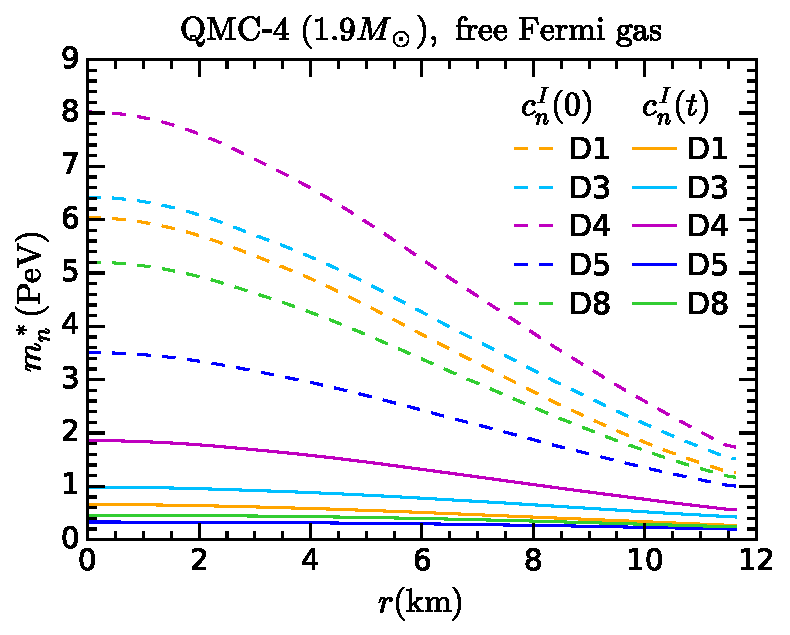
\includegraphics[width=0.495\textwidth]{capture_3/mnstar_r_QMC4_free_Fermi.pdf}    
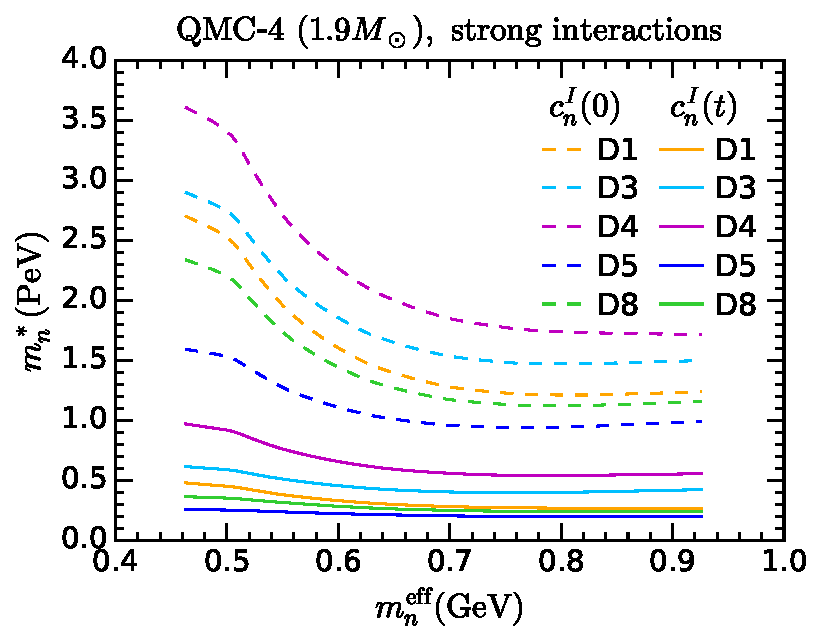
\includegraphics[width=0.495\textwidth]{capture_3/mnstar_mn_QMC4.pdf}
    \caption{Radial profiles of $\mnstar$ in the free Fermi gas approach (left) and $\mnstar$ as a function of the neutron effective mass (right) in the interacting baryon approach, for selected operators. We assume the NS configuration QMC-4 ($1.9\Msun$). In both cases, $\mnstar$ has been calculated using neutron couplings at zero momentum transfer (dashed lines) and including the dependence on $t$ (solid lines). }
    \label{ch5:fig:mstar}
\end{figure}
%%%%%%%%%%%%%%%%%%%%%%%%%%%%%%%%%%%%%


In the left panel of Fig.~\ref{ch5:fig:mstar}, we show radial profiles of $\mnstar$ for five representative operators in the case of a QMC-4 NS. These profiles have been calculated in the free Fermi gas approximation (i.e. the neutron mass remains constant throughout the star) both with (solid lines) and without (dashed lines) including the momentum-dependent neutron form factors $c_n^I(t)$. 
The profiles illustrate the variation of $\mnstar$ with $B(r)$ and $\kinFn(r)$ in the stellar interior. Note that $\mnstar$ also depends on the  DM velocity distribution, which we have taken to be Maxwell-Boltzmann. We can see that the inclusion of $t$-dependent neutron couplings lowers $\mnstar$ by a factor of $\sim 1.2 - 4.5$, with D4 and D3 being less affected. 
This is because of the suppression of large energy transfers when introducing  $c_i^I(t)$ (as illustrated in Fig.~\ref{ch5:fig:intrateqtr1}) which results in less energy being lost by the DM particle per collision.  A lower value of $\mnstar$ means that multiple scattering is relevant at smaller DM masses than those expected with $c_i^I(0)$. 

In the interactive baryon approach, $\mnstar$ is also a function of $\mneff(r)$, as plotted in the right hand panel of Fig.~\ref{ch5:fig:mstar}. 
The values of $B(r)$, $\kinFn(r)$, and $\mneff(r)$ used in the right-hand panel are those corresponding to the appropriate radial coordinate within the NS as in the left-hand panel. 
In this case, when including the dependence on the transferred momentum (solid lines), $\mnstar$ is reduced by a factor of $\sim 1.2 - 2.5$ compared the result obtained with hadronic matrix elements at zero momentum transfer (dashed lines). Thus, multiple scattering is relevant at an even lower DM mass in the complete approach that accounts both for strong interactions and $t$-dependent nucleon couplings. 
The remaining operators show a similar behaviour to those presented in Fig.~\ref{ch5:fig:mstar}.


\section{Capture Rate Results}
\label{ch5:sec:capture_results}
%%%%%%%%%%%%%%%%%%%%%%%%%%%%%%%%%%%%%%%%%%%%%%%%%%%%%%%%%%%%%%%%%%%%%
%%%%%%%%%%%%%%%%%%%%%%%%%%%%%%%%%%%%%%%%%%%%%%%%%%%%%%%%%%%%%%%%%%%%%

In this section, we present our results for the capture rate, 
for each EFT operator in Table~\ref{ch1:tab:opers_defn_full} and every baryonic species in the QMC family. The rates have been calculated in the optically thin limit using Eq.~\ref{ch5:eq:cap_general} for $m_\chi\lesssim \mstar$ and with same equation but including the capture probability $c_1(r)$ in the interaction rate for $m_\chi\gtrsim \mstar$ wherever the target is degenerate, and Eq.~\ref{ch5:eq:capture_simple} in the non-degenerate regime\footnote{We have numerically evaluated these equations using the \texttt{CUBA} libraries \cite{Hahn:2004fe_CUBALibrarymultidimensional,Hahn:2014fua_Concurrentcuba} linked to \texttt{Mathematica}~\cite{Mathematica}.}. We compute the capture rate for each target species individually as these can be summed to obtain the total capture rate. Since we shall always work in the optically thin limit (i.e., where the probability for more than one scattering interaction per DM orbit is very low) this procedure is a good approximation, even in the multi-scattering mass region.
We assume a NS located in the Solar neighbourhood, thus $\rho_\chi=0.4\GeV\cm^{-3}$, $\vstar=230\km\s^{-1}$ and $v_d=270\km\s^{-1}$.  



%%%%%%%%%%%%%%%%%%%%%%%%%%%%%%%%%%%%%%%%%%%%%%%%%%%%%%%%%%%%%%%%%%%%%%%%%%%%%%%%%%%%
\subsection{Nucleons}
\label{sec:capresnucleons}
%%%%%%%%%%%%%%%%%%%%%%%%%%%%%%%%%%%%%%%%%%%%%%%%%%%%%%%%%%%%%%%%%%%%%%%%%%%%%%%%%%%%

%%%%%%%%%%%%%%%%%%%%%%%%%%%%%%%%%%%%%%%
\begin{figure}[t!bp] 
\centering
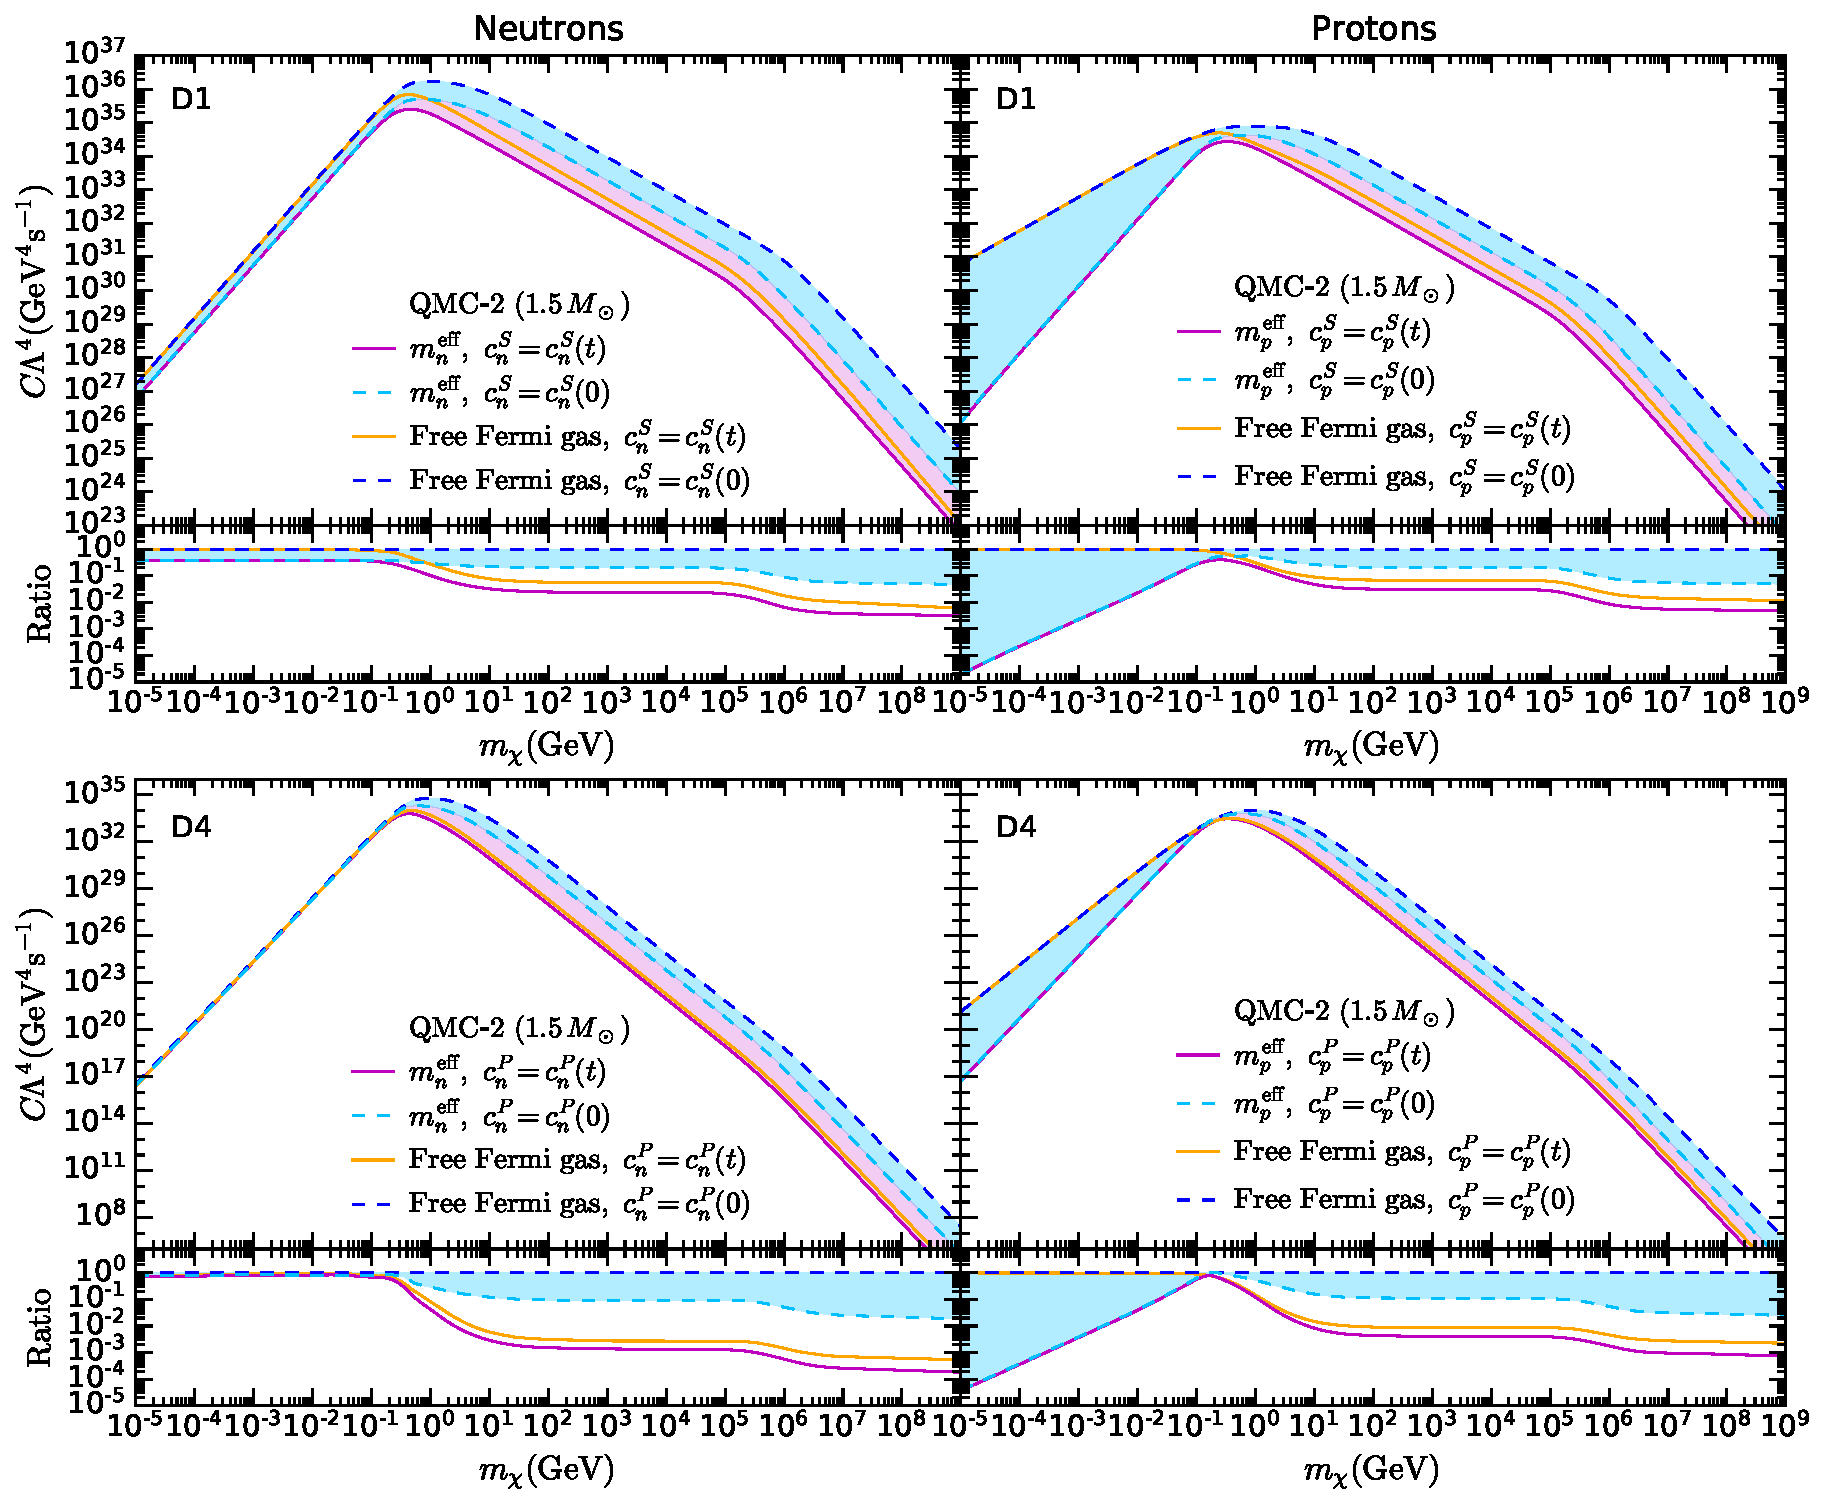
\includegraphics[width=\textwidth]{capture_3/C_mDM_N_QMC_D1_D4_ratio.pdf}
\caption{
Capture rate in the optically thin limit for the operators D1 (top) and D4 (bottom) as a function of the DM mass $m_\chi$ for neutron (left) and proton (right) targets, for a QMC-2 NS configuration.  We compare the free Fermi gas approach with constant nucleon couplings (dashed blue) and momentum-dependent couplings (solid orange), and the interacting nucleon approach for constant couplings (dashed light blue) and momentum-dependent couplings (solid magenta). Note that these rates scale as $\Lambda^{-4}$. 
The ratio of the capture rate compared to that for the free Fermi gas approximation for point-like targets (dashed dark blue, as computed in Chapter~\ref{chapter:capture_intro}) is shown in the lower panels. 
}
\label{ch5:fig:capratesD1D4}
\end{figure} 
%%%%%%%%%%%%%%%%%%%%%%%%%%%%%%%%%%%%%%%

%%%%%%%%%%%%%%%%%%%%%%%%%%%%%%%%%%%%%%%
\begin{figure}[t!bp] 
\centering
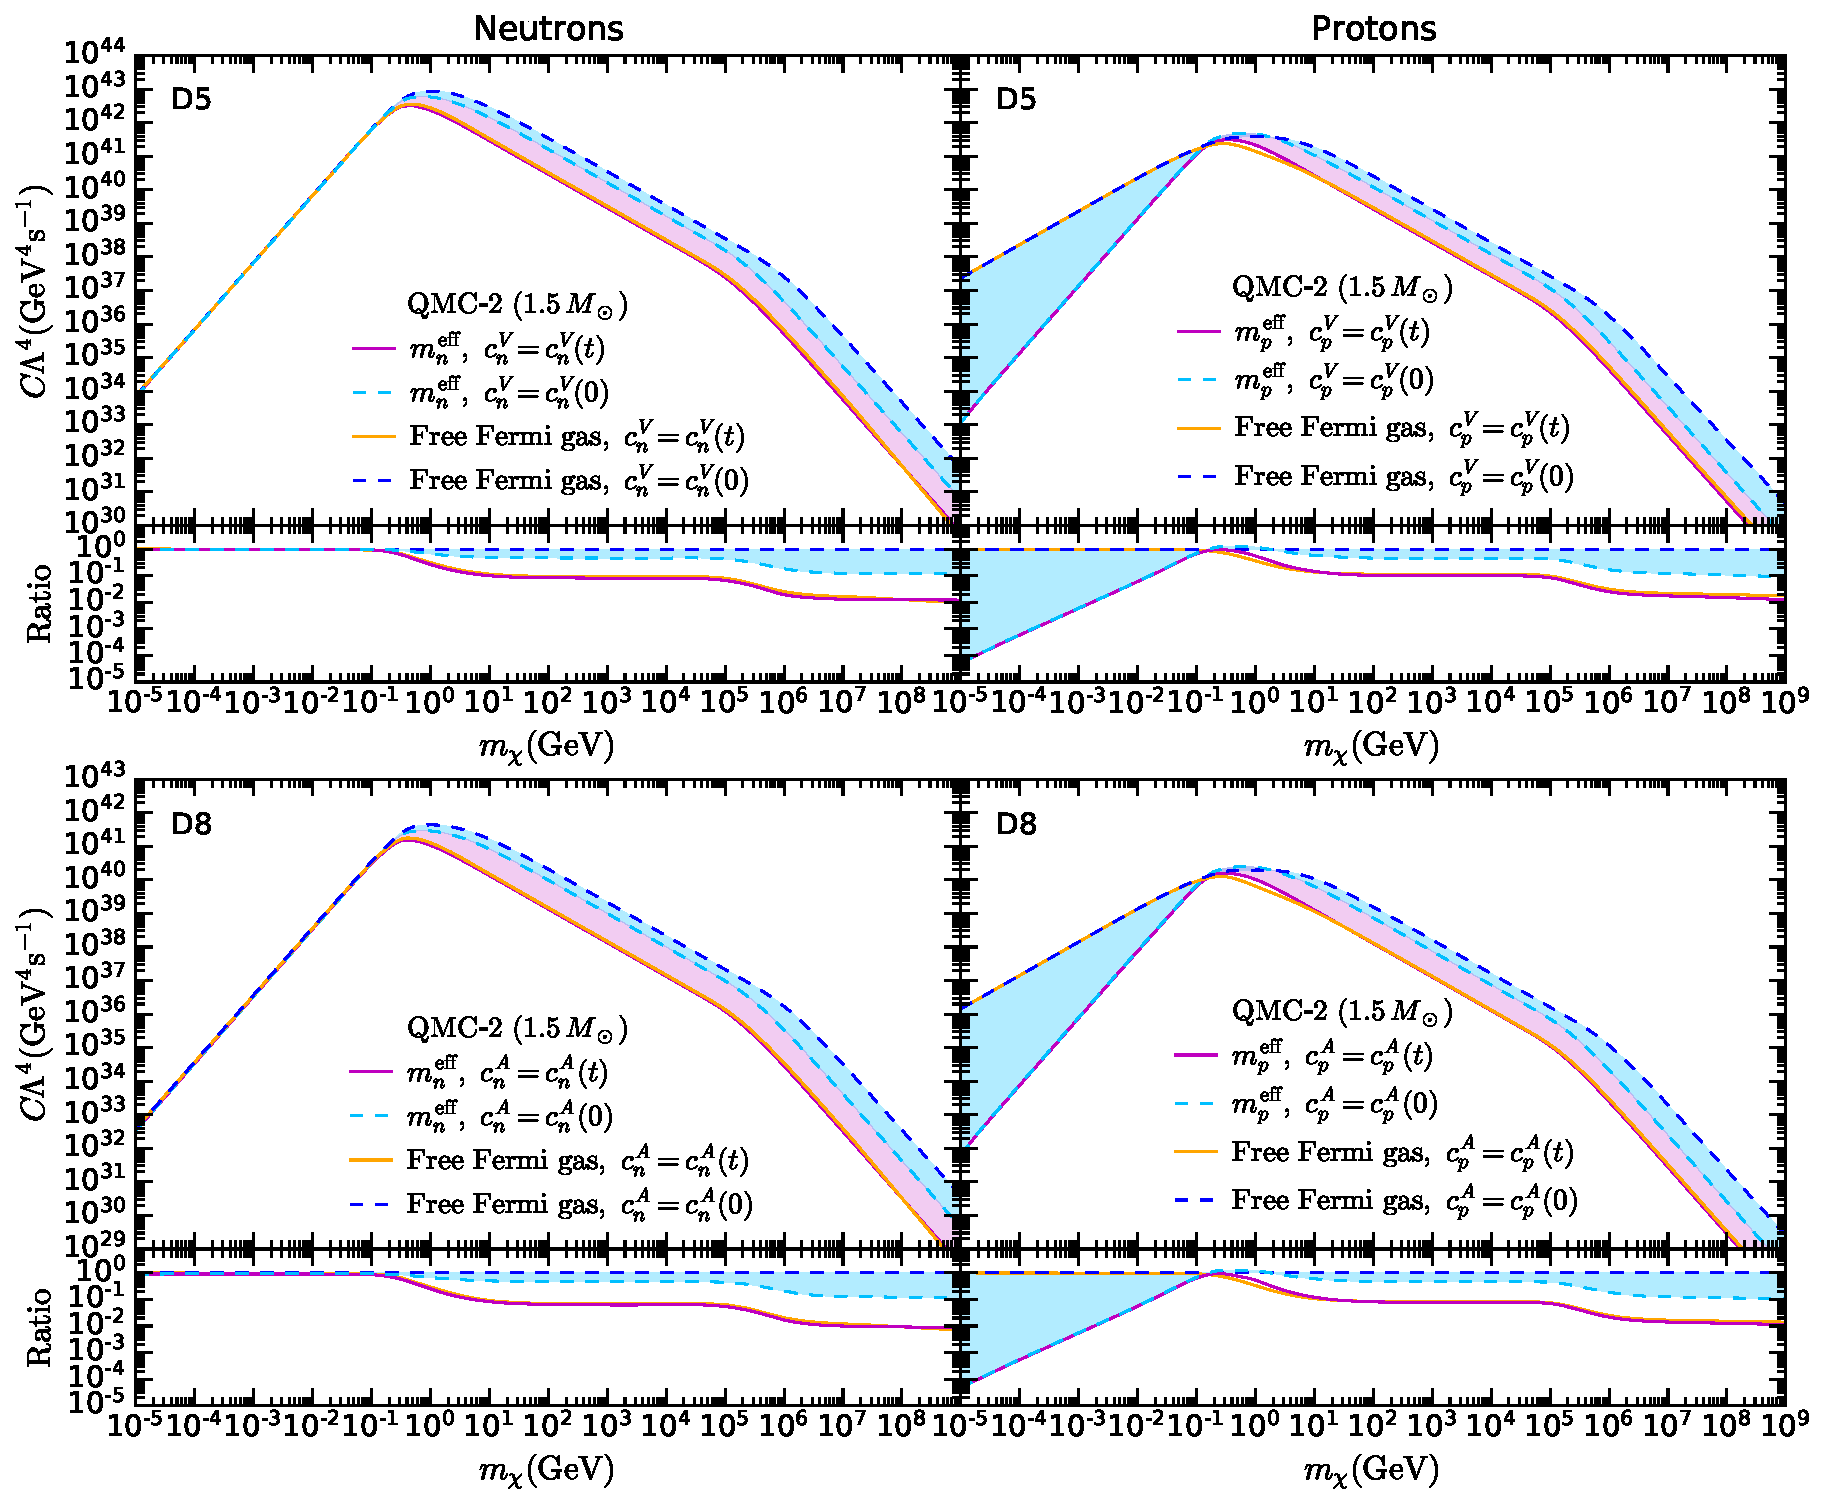
\includegraphics[width=\textwidth]{capture_3/C_mDM_N_QMC_D5_D8_ratio.pdf}
\caption{
Capture rate in the optically thin limit for the operators D5 (top) and D8 (bottom) as a function of the DM mass $m_\chi$ for neutron (left) and proton (right) targets,
using the free Fermi gas approach with constant nucleon couplings (dashed blue) and momentum-dependent couplings (solid orange), and the interacting nucleon approach for constant couplings (dashed light blue)  and momentum-dependent couplings (solid magenta), for a QMC-2 NS configuration. 
Note that these rates scale as $\Lambda^{-4}$. 
The ratio of the capture rate compared that for the free Fermi gas approximation for point-like targets (dashed dark blue) is shown in the lower panels. 
}
\label{ch5:fig:capratesD5D8}
\end{figure} 
%%%%%%%%%%%%%%%%%%%%%%%%%%%%%%%%%%%%%%%

To illustrate the effect of accounting for strong interactions and th emomentum dependence of the nucleon couplings, we show in  Figs.~\ref{ch5:fig:capratesD1D4} and \ref{ch5:fig:capratesD5D8} the capture rate for four representative operators, D1, D4, D5, and D8, for a QMC-2 NS configuration ($1.5\Msun$). 
Note that in these figures we have not assumed a value of $\Lambda$, i.e. we plot $C \Lambda^4$. 
Results are shown for the free Fermi gas approximation with constant nucleon couplings (dashed dark blue) and momentum dependent form factors (orange), and for the interacting baryon framework with (magenta) and without (dashed light blue) $t$-dependent nucleon couplings.
 

For neutron targets in the free Fermi gas approach, we find that including momentum-dependent form factors in the scattering cross-section does not affect the capture rate for DM masses $m_\chi\lesssim0.2\GeV$, since the energy scale at which this effect comes into play is $Q_0\sim1\GeV$. For $m_\chi\gtrsim1\GeV$, the ratio of the calculation that accounts for $t$-dependent neutron couplings compared to that obtained with constant hadronic matrix elements is ${\cal O}(10^{-2})$ 
for D4 in the large DM mass range; for the remaining operators the suppression exceeds one order of magnitude.

The fact that this effect is stronger for operators whose matrix elements are a function of larger powers of $t$, such as D4, can be seen from  Eq.~\ref{ch5:eq:capture_simple}, where we note that 
$\mathcal{F}_n$ is a decreasing function of $n$. 
We also note that the suppression caused by the form factors is stronger in the multiple scattering regime, $m_\chi\gtrsim\mnstar$, because the values of $\mnstar$ become lower when $t$-dependent neutron couplings are introduced (see Fig.~\ref{ch5:fig:mstar}, left panel). As mentioned above, this is a consequence of the form factors imposing a cutoff on the 
size of the momentum transfer in the capture process, hence lowering the average DM energy loss per scattering. 
It is worth remarking that the suppression caused by the momentum dependence of the form factors is even more pronounced in heavier NSs where higher momentum transfers are possible~\cite{Bell:2020obw_sep_NucleonStructureStrong}. 

Similar conclusions are obtained for DM capture associated with scattering from protons (right panels), where the suppression of the capture rate is slightly smaller than that for neutrons. 
As previously stated, we have taken $Q_0=0.9\GeV$ as a conservative choice; smaller values of $Q_0$ will result in a stronger suppression of the capture rate. 


We now turn to the effect of strong interactions on the capture process. For $m_\chi\lesssim 0.2\GeV$, the DM mass range where Pauli blocking is in effect, the capture rate due to DM-neutron scattering is almost identical for the free Fermi gas (dashed dark blue) and interacting baryon (dashed light blue) approaches, for operators D3-D10. This is because capture occurs very close to the NS surface. Operators D1 and D2 suffer a relatively small overall rescaling, because their interaction rates scale with the neutron mass, in this case $(\mneff)^2$. 


For protons, however, there is a significant difference in the capture rate in the low DM mass range. In the free Fermi gas approach, protons are degenerate only in the innermost region of the NS core, with the exact extent of that region dependent on the NS configuration (see Fig.~\ref{ch5:fig:muradprofs}, dashed lines).  For the particular NS model QMC-2, proton targets are affected by Pauli blocking only within a radius of $\sim4\km$ from the NS centre. Consequently, in the free Fermi gas approach (dashed dark blue) the capture rate for scattering on protons is not Pauli suppressed at low DM mass, in contrast to that for neutrons; see the different slope of the capture rates at $m_\chi\lesssim m_p$.
As a result, capture on proton targets surpasses the contribution of the dominant species, neutrons, in the free Fermi gas approximation and light DM mass regime. 

However, in the interacting baryon approach, protons are degenerate over a much wider region of the stellar interior (see Fig.~\ref{ch5:fig:muradprofs}, solid lines). Therefore, the more accurate interacting baryon approach leads to much greater Pauli suppression of the capture rate for scattering on protons. Indeed, the proton contribution to the total capture rate is lower than that of neutrons in most cases. In the case of a QMC-2 NS configuration, the sole exception is for the operator D4. Therefore,  the ratio of capture rates for the free Fermi gas and interacting baryon approaches is largest for the scattering of light DM on protons, and exceeds 4 orders of magnitude at $m_\chi=10\keV$, for all operators. 


For DM masses above $m_\chi\sim m_n$, the capture rate in the interacting baryon framework and with constant nucleon couplings is lower by up to one order of magnitude compared to that for the free Fermi gas approach, for both neutron and proton targets for operators D1-4.
For the remaining operators, the suppression reaches the $\sim30\%$ level in the large DM mass region. 
Note that the capture rate depends on the DM-target reduced mass, which for $m_\chi\gg m_i$ is approximately target mass. Furthermore, in this mass regime, DM capture can occur deep inside the star, where $\mbeff<m_i$, hence the capture rate is suppressed by a lower target mass.

Introducing momentum-dependent form factors in the interacting baryon approach (magenta lines) results in a similar reduction of the capture rate to that of the ideal Fermi gas formalism (orange lines), especially for operators D5-D10. For operators D1-D4, the capture rate is lowered by $\sim3$ orders of magnitude in the multiple scattering regime for both neutron and proton targets. 


It is worth noting that the combined effect of using the interacting baryon approach and including momentum-dependent form factors is smaller than the product of the two individual effects. This is because the form factor suppression $\mathcal{F}_n$ in Eq.~\ref{ch5:eq:capture_simple} is a decreasing function of the target mass, which can reach values as small as $\mneff\sim0.5m_n$ for nucleon targets, thereby resulting in a weaker reduction of the capture rate when compared to the free Fermi gas approach. 

% In Appendix~\ref{sec:uncereos}, we have compared  our results for the QMC EoS with those for the BSk24 functional~\cite{Goriely:2013,Pearson:2018tkr}  (a Skyrme type EoS).  We find that the size of the effects described above are largely independent of the EoS.




%%%%%%%%%%%%%%%%%%%%%%%%%%%%%%%%%%%%%%%%%%%%%%%%%%%%%%%%%%%%%%%%%%%%%%%%%%%%%%%%%%%%
\subsubsection{Hyperons}
\label{sec:capresexotic}
%%%%%%%%%%%%%%%%%%%%%%%%%%%%%%%%%%%%%%%%%%%%%%%%%%%%%%%%%%%%%%%%%%%%%%%%%%%%%%%%%%%%

%%%%%%%%%%%%%%%%%%%%%%%%%%%%%%%%%%%%%%%%
\begin{figure}[t!bp] 
\centering
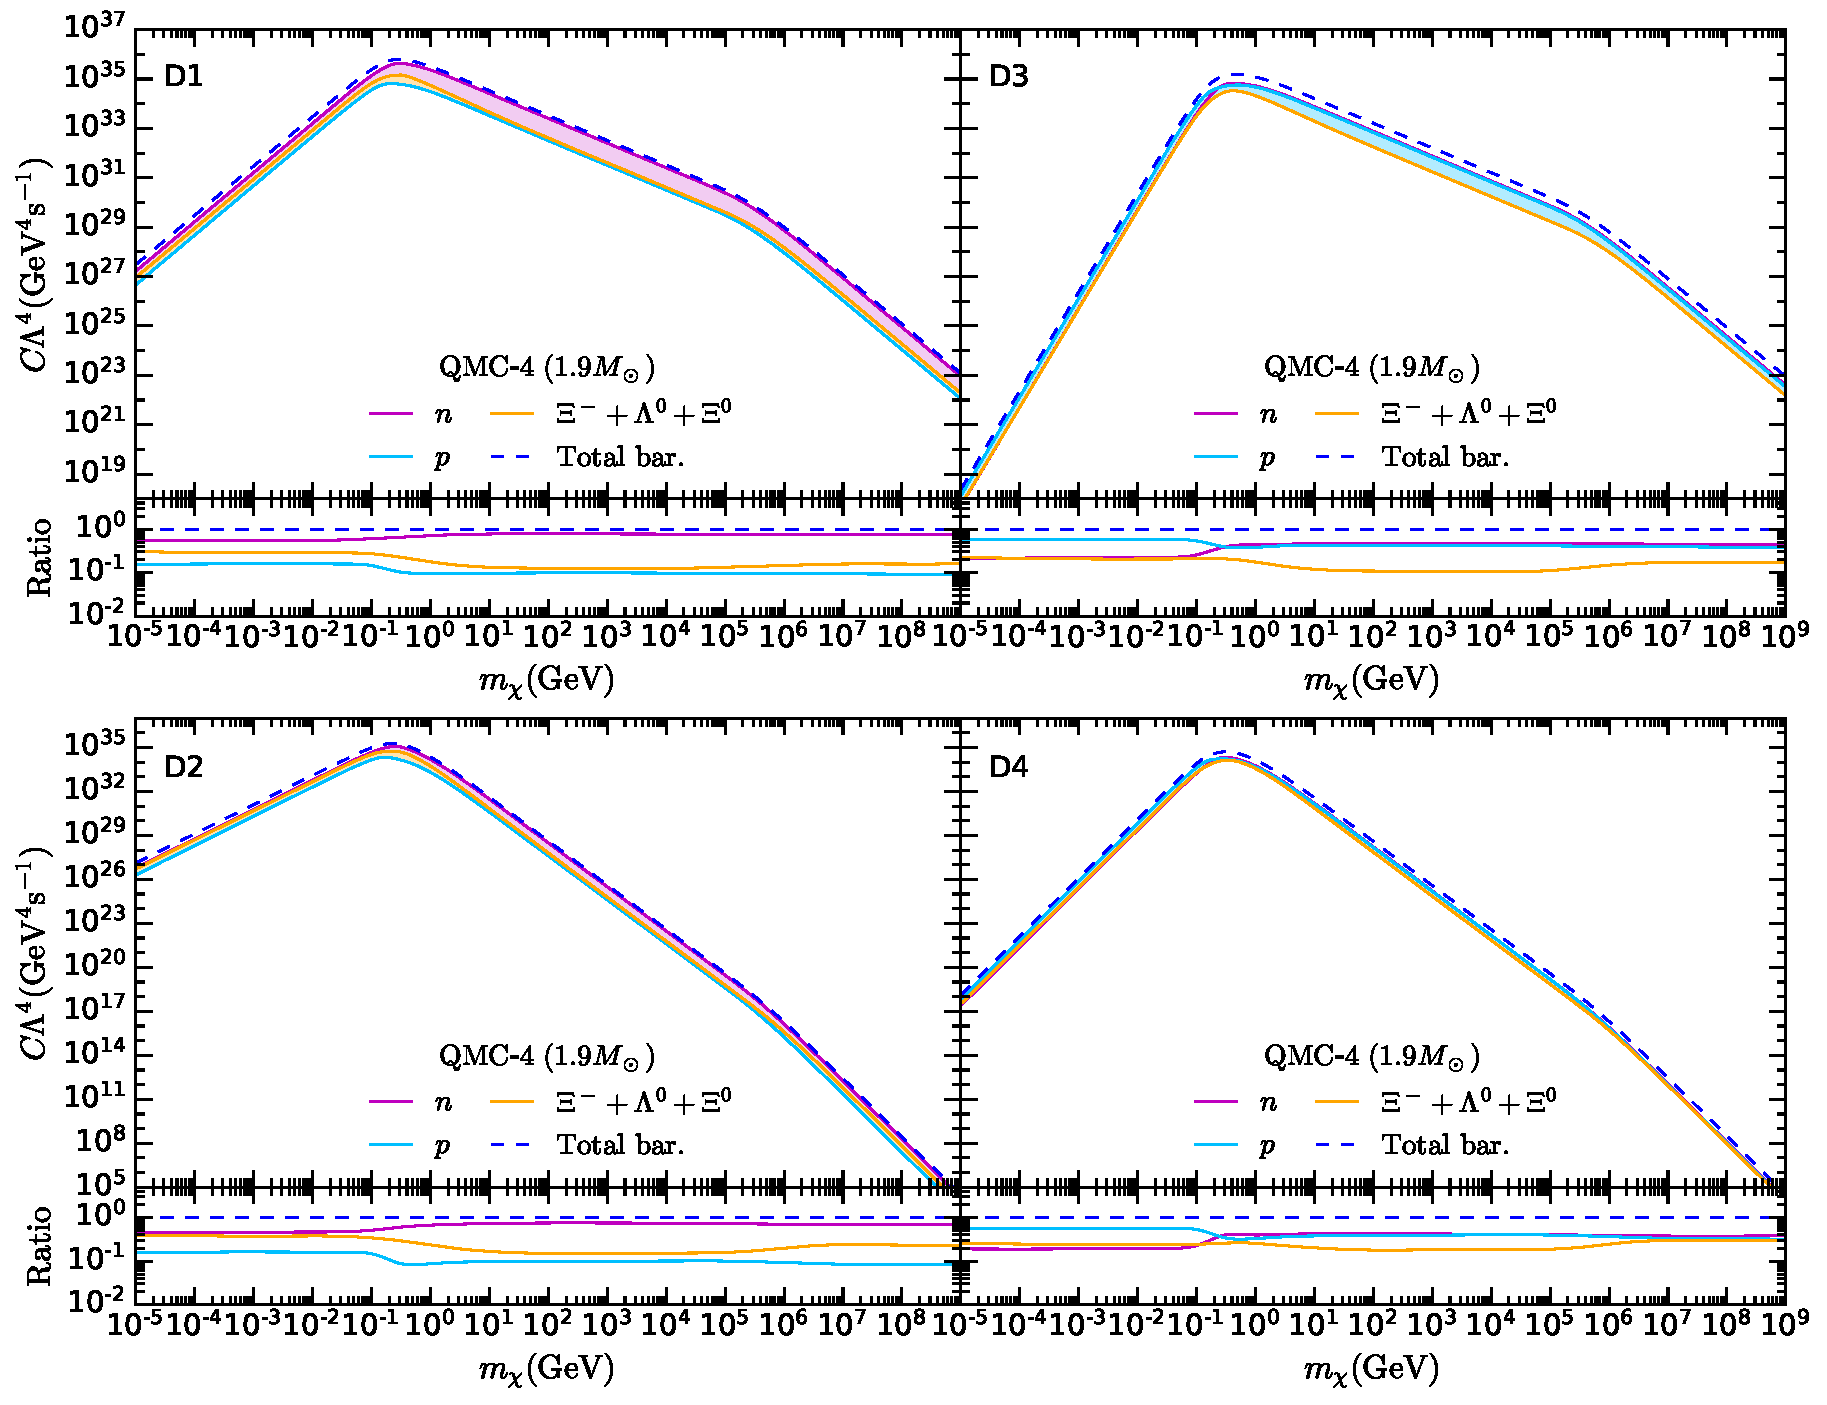
\includegraphics[width=\textwidth]{capture_3/D1_D4_C_mDM_hyper_meff_ratio.pdf}
\caption{Capture rate in the optically thin limit for operators D1-D4 as a function of the DM mass $m_\chi$ for nucleons and exotic targets in the NS benchmark configuration QMC-4 ($1.9\Msun$). All capture rates were calculated using the complete approach that accounts for strong interactions and momentum-dependent form factors for baryons. Note that these rates scale as $\Lambda^{-4}$. The lower panels show the contribution of each baryonic species to the total capture rate associated with DM interactions with baryons (dashed blue line). 
}
\label{ch5:fig:capratesD1D4_Hyper}
\end{figure}  
%%%%%%%%%%%%%%%%%%%%%%%%%%%%%%%%%%%%%%%%



In Figs.~\ref{ch5:fig:capratesD1D4_Hyper} and~\ref{ch5:fig:capratesD5D10_Hyper}, we show the capture rates $C \Lambda^4$ for all the baryonic species in the benchmark NS QMC-4, calculated using the interactive baryon framework with momentum dependent DM couplings. As outlined in section~\ref{ch2:subsec:NS_EoS}, the NS configuration QMC-4 contains $\Lambda^0$, $\Xi^-$ and $\Xi^0$ hyperons in the inner core.  
The orange line represents the sum of the capture rate due to scattering on all the hyperonic species. Their individual contributions are determined by their abundance in the NS core (see Fig.~\ref{ch2:fig:QMC_profiles}, bottom left panel) and hence $\Xi^-$ and $\Lambda^0$ give sizeable contributions to the capture rate while that of $\Xi^0$ is negligible. 


For operators D1 and D5-D10, scattering on neutrons (magenta) clearly dominates the total capture rate (dashed dark blue) throughout the whole DM mass range considered here, followed by protons (light blue) and hyperons. 
For D3 and D4, proton targets provide the largest contribution to the capture rate in the Pauli blocked region $m_\chi\lesssim0.2\GeV$. This occurs because of an interesting interplay of two effects. First, close to the surface of the star, the proton Fermi energy is lower than that of neutrons (see Fig.~\ref{ch5:fig:muradprofs}, solid lines). In fact, the proton contribution to the total capture rate is the largest in the light DM mass regime for all operators. 
Second, operators whose matrix elements are a function of larger powers of $t$ (such as D3 and D4) are more affected by Pauli blocking. As such, the neutron contribution is more suppressed for these operators. 

%%%%%%%%%%%%%%%%%%%%%%%%%%%%%%%%%%%%%%%%
\begin{figure}[t!bp] 
\centering
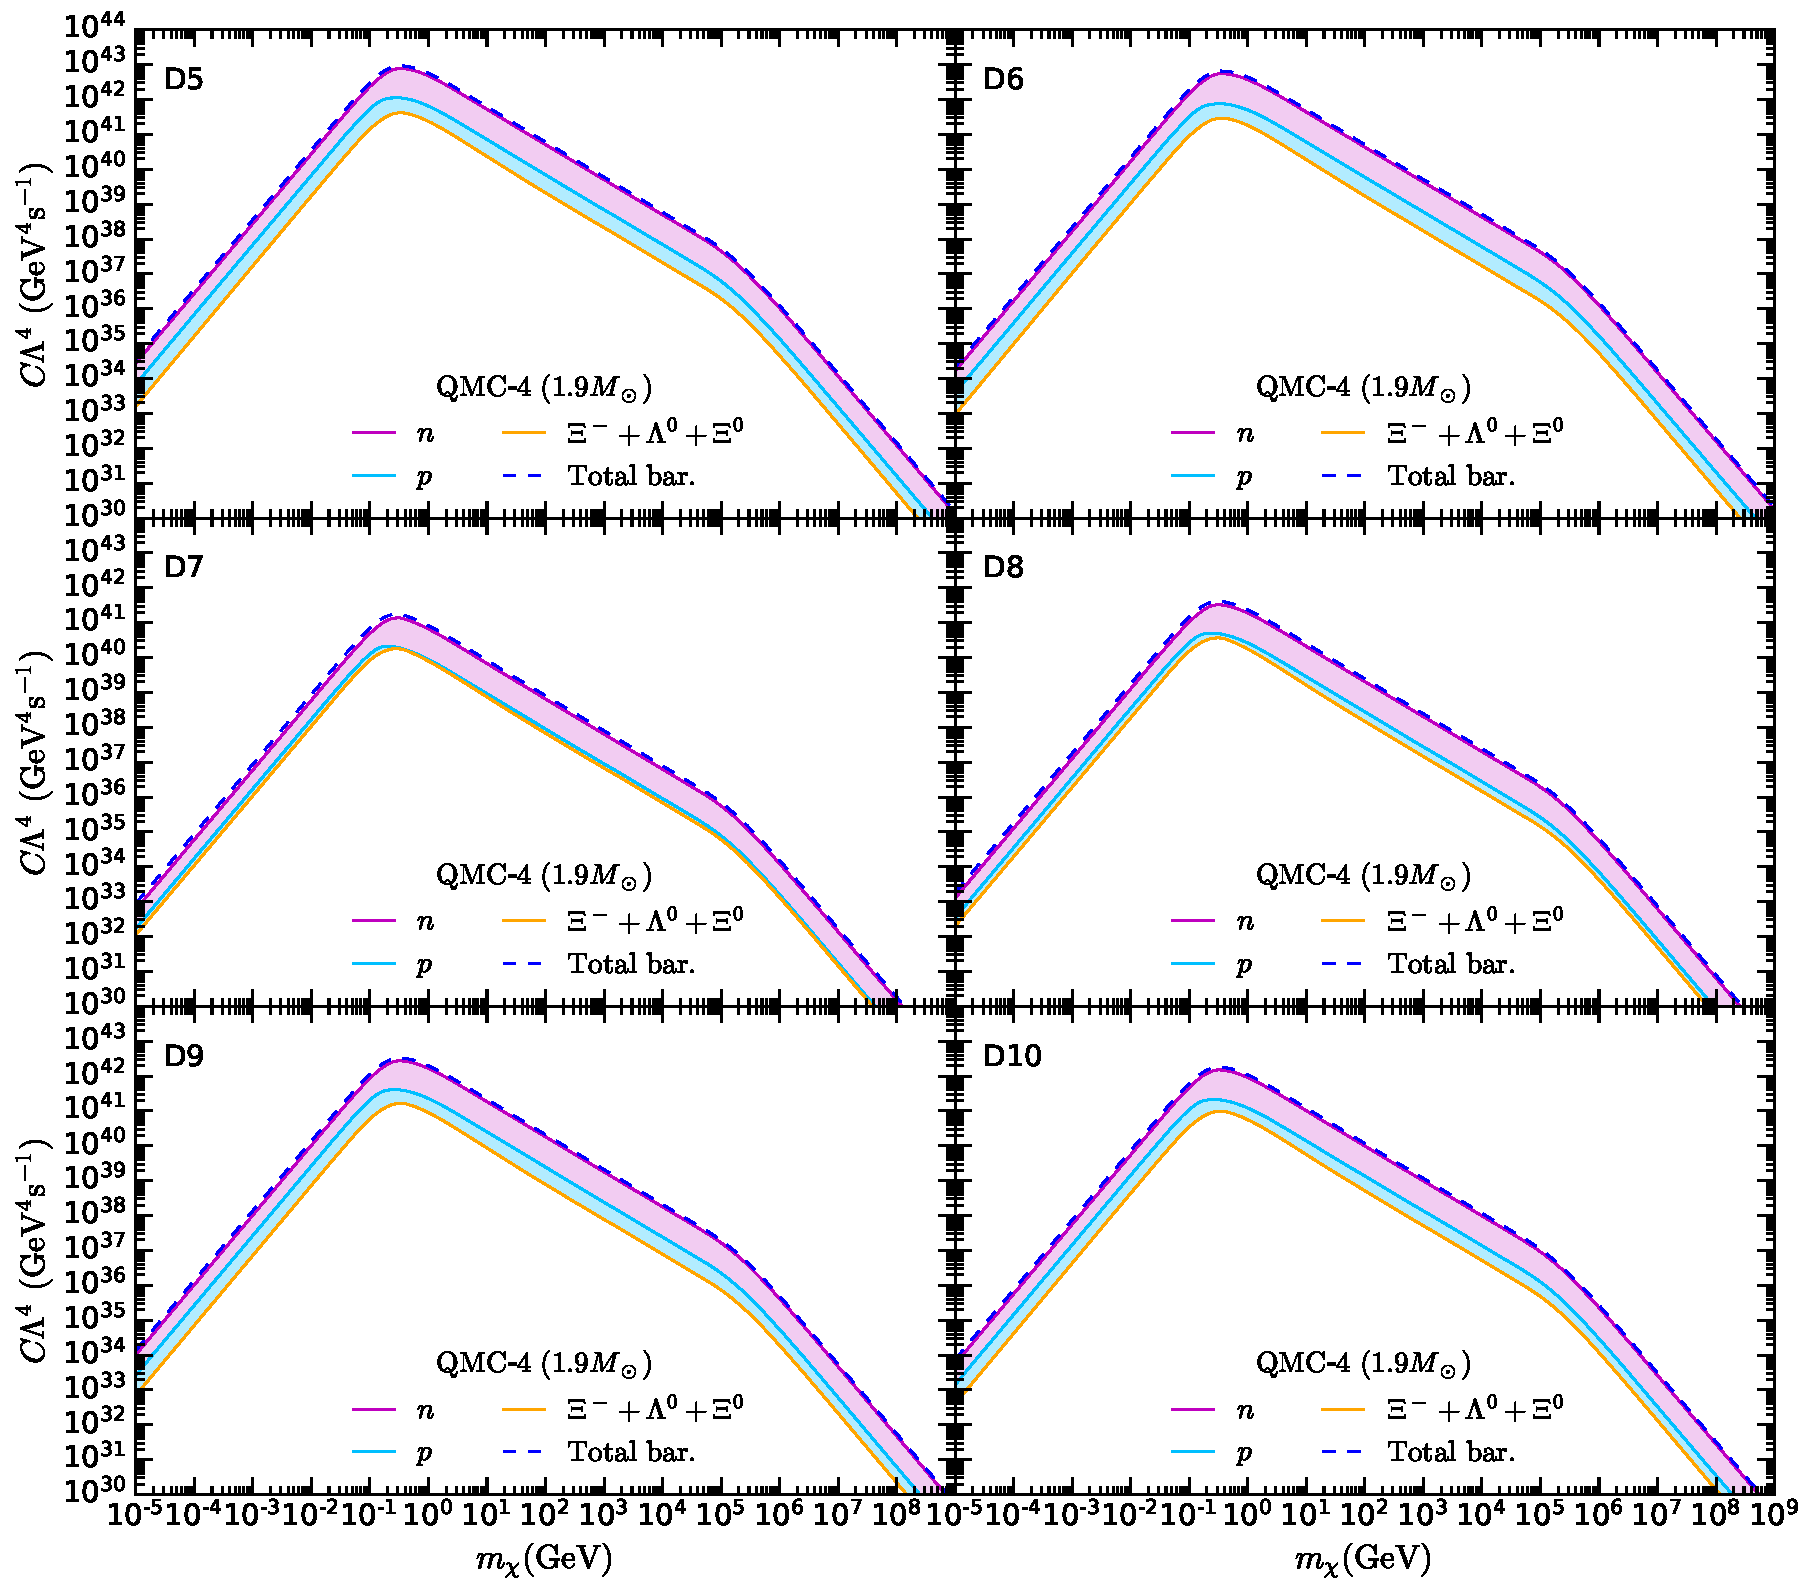
\includegraphics[width=\textwidth]{capture_3/D5_D10_C_mDM_hyper_meff.pdf}
\caption{Capture rate in the optically thin limit for operators D5-D10 as a function of the DM mass $m_\chi$ for nucleons and exotic targets in the NS benchmark configuration QMC-4 ($1.9\Msun$). All capture rates were calculated using the complete approach that accounts for strong interactions and momentum-dependent form factors for baryons. Note that these rates scale as $\Lambda^{-4}$. 
}
\label{ch5:fig:capratesD5D10_Hyper}
\end{figure}  
%%%%%%%%%%%%%%%%%%%%%%%%%%%%%%%%%%%%%%%%

For D3 and D4, the capture rates due to scattering on the three species, neutrons, protons, and hyperons, are all of similar magnitude when $m_\chi\gtrsim0.2\GeV$. In fact, hyperons surpass the neutron contribution for D4, especially in the multiple scattering regime.  Recall that hyperon effective masses are much larger than the nucleon masses in the inner core (see Fig.~\ref{ch2:fig:QMC_profiles}, bottom right panel). Thus, despite being under-abundant, their contribution to the capture rate is enhanced by a larger DM-target reduced mass and by the D4 matrix element being $\Msq\propto t^2$ ($n=2$ in  Eq.~\ref{ch5:eq:capture_simple}). 

For D2-D4, the capture rates due to scattering on neutrons and hyperons are almost identical for $m_\chi\lesssim0.1\GeV$, with hyperons once again surpassing neutrons in the particular case of D4.  This occurs because the depth of the Fermi sea of hyperons is much lower than that of the neutrons in the NS core, thus leading to less Pauli blocking. 

In addition, we have compared these results with those for a NS configuration of very similar compactness to that of QMC-4, but obtained with a QMC model that does not contain hyperons. We have found that the total capture rate due to DM interactions with baryons for operators D2-D4 is enhanced by the presence of hyperonic matter in the NS core. For D3 and D4, this enhancement reaches a factor of $\sim 2$ and $\sim 3$, respectively.


%%%%%%%%%%%%%%%%%%%%%%%%%%%%%%%%%%%%%%%%%%%%%%%%%%%%%%%%%%%%%%%%%%%%%
%%%%%%%%%%%%%%%%%%%%%%%%%%%%%%%%%%%%%%%%%%%%%%%%%%%%%%%%%%%%%%%%%%%%%
\section{Threshold Cross-Sections for Nucleon Scattering}
\label{ch5:sec:sigmath_results}
%%%%%%%%%%%%%%%%%%%%%%%%%%%%%%%%%%%%%%%%%%%%%%%%%%%%%%%%%%%%%%%%%%%%%
%%%%%%%%%%%%%%%%%%%%%%%%%%%%%%%%%%%%%%%%%%%%%%%%%%%%%%%%%%%%%%%%%%%%%



In Section~\ref{ch3:subsec:geom_lim_threshold_xs}, we defined the threshold cross-section $\sigmathi$ for a given target, $i$, as the cross-section for which the capture rate in the optically thin regime $C(m_\chi,\sigma(m_\chi,\Lambda))$ reaches the geometric limit, $C_\mathrm{geom}$. Above this threshold, the capture rate saturates to $C_\mathrm{geom}$, and hence $\sigma = \sigmathi$ cannot be distinguished from $\sigma\ge\sigmathi$. For the intermediate DM mass range where NS capture is most efficient, i.e., where neither Pauli blocking nor multiscattering are relevant, a value of $\sigmathn = \textrm{few}\times10^{-45}\cm^2$ is commonly assumed in the literature.  However, as we shall see the combined effects of nucleon interactions and momentum dependence of the hadronic matrix elements imply that the true value is somewhat larger. 


In Fig.~\ref{ch5:fig:sigmathcomp}, we show the impact of accounting for both strong interactions and nucleon structure on the threshold cross-section for both neutrons (left) and protons (right). This is done for operators D1 (top) and D8 (bottom) in the benchmark NS QMC-2 ($1.5\Msun$). The dashed lines represent the results obtained in the free Fermi gas approximation, which yields $\sigmathn\simeq2\times10^{-45}\cm^2$ in the $1\GeV\lesssim m_\chi\lesssim 4\times 10^5\GeV$ range and $\sigmathp\simeq2\times10^{-44}\cm^2$ in a similar DM mass range for both operators. Below $m_\chi\sim1\GeV$ the NS sensitivity is suppressed by Pauli blocking, while multiple scattering comes into play above $m_\chi\sim4\times10^5\GeV$. 

When the corrections for nucleon structure and strong interaction are introduced (solid lines), the region of constant sensitivity is reduced to $100\GeV\lesssim m_\chi\lesssim  10^5\GeV$ and the value of the threshold cross-section is no longer the same for D1 and D8. This discrepancy is due to the nucleon couplings for the scalar operators (D1-4) being proportional to the nucleon mass, which induces a larger suppression in the capture rate for D1 compared to D8. In this DM mass regime, we find $\sigmathn\simeq3.6\times10^{-44}\cm^2$ for D1 and $\sigmathn\simeq1.4\times10^{-44}\cm^2$  for D8. For protons, the DM sensitivity is also lowered by a similar amount. In the multi-scattering regime, for both targets, we observe an even more pronounced effect, with $\sigmathn$ reaching a factor of $\sim52 \,(20)$ larger than in the ideal Fermi gas approach for D1 (D8), and $\sigmathp$  a factor of $\sim 35 \,(16)$. 

%%%%%%%%%%%%%%%%%%%%%%%%%%%%%%
\begin{figure}[t!bp]
   \centering
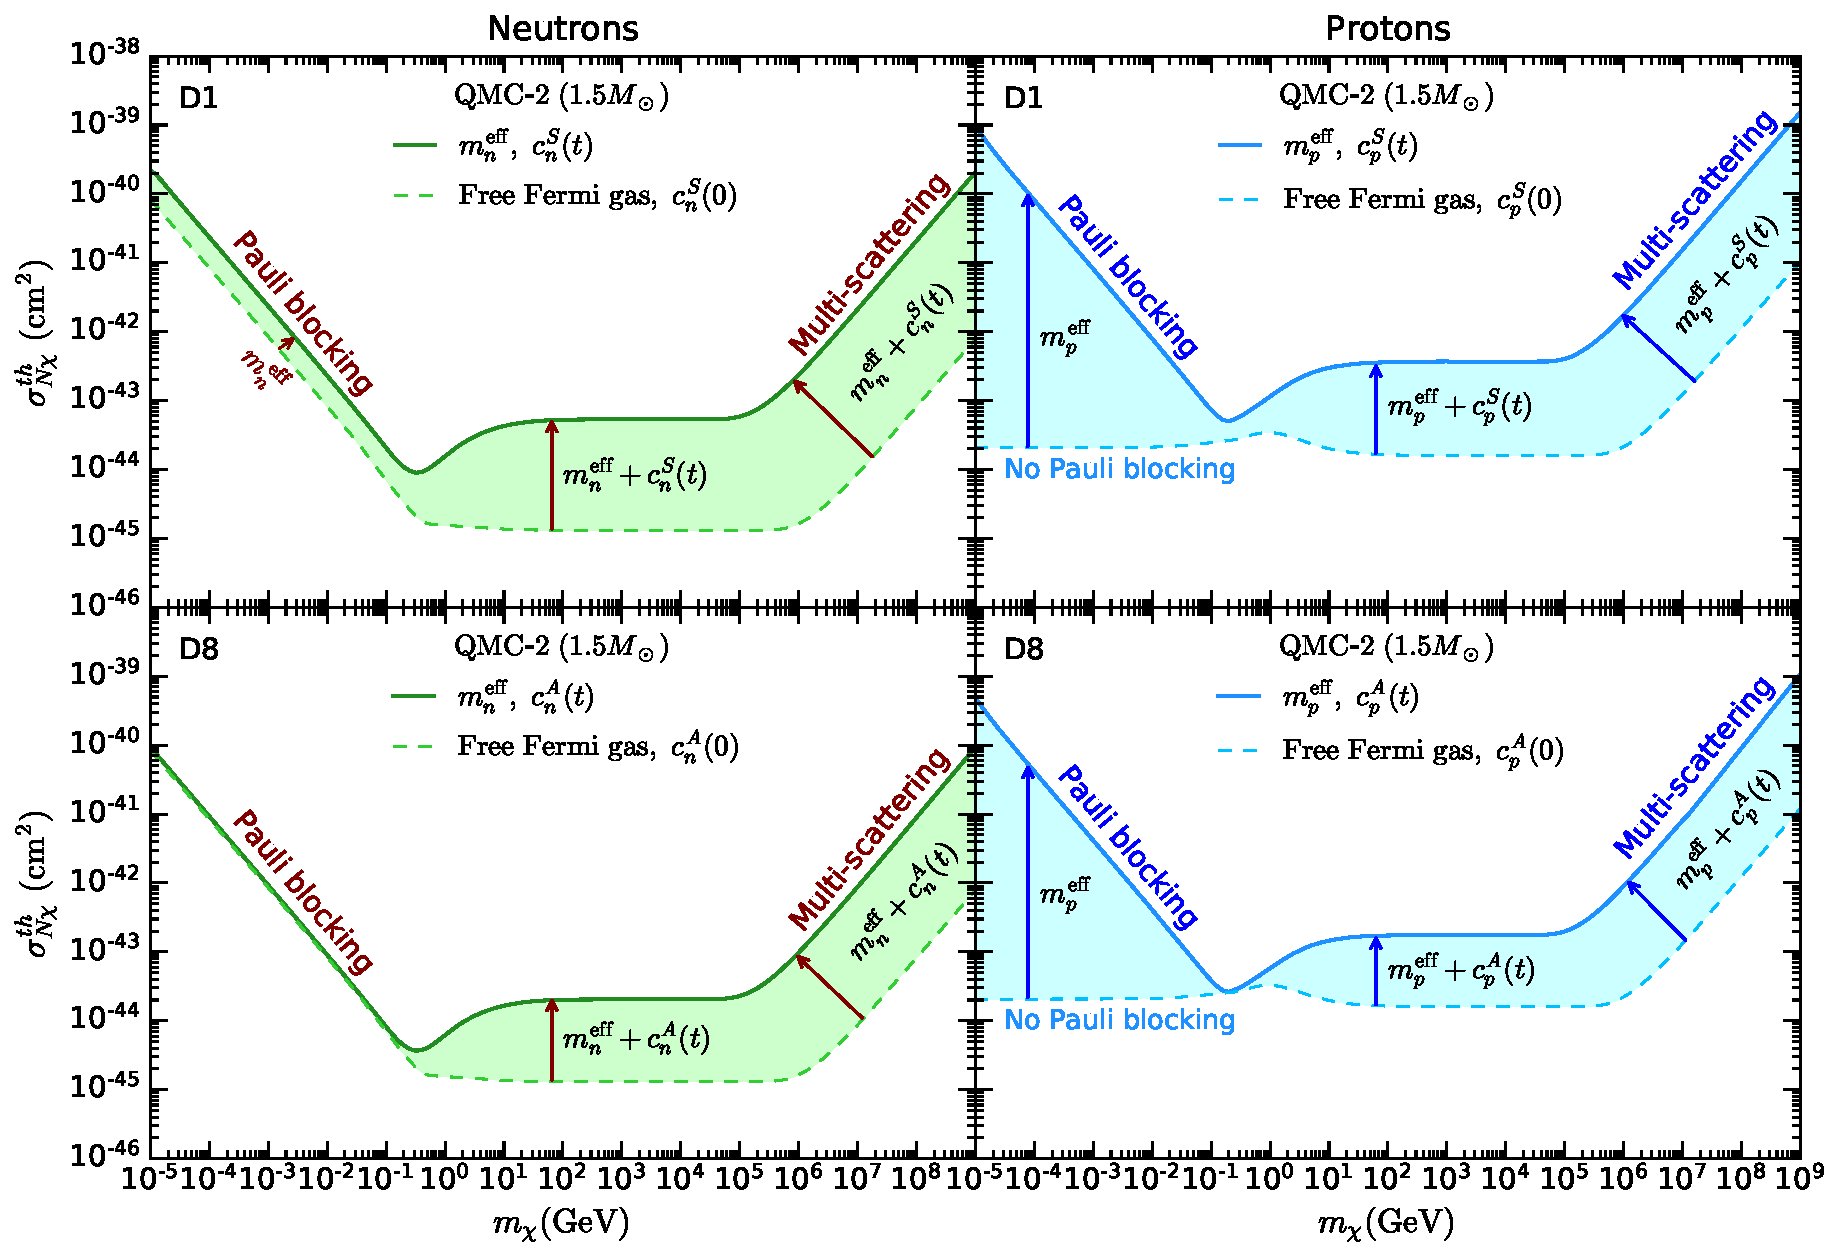
\includegraphics[width=\textwidth]{capture_3/sigmath_N_D1_D8.pdf}
\caption{Threshold cross-section for neutron (left) and proton (right) targets with scalar-scalar (D1, top) and axial-axial (D8, bottom) interactions with DM in a QMC-2 ($1.5\Msun$) NS. 
The solid lines represent the result obtained using the interacting baryon framework ($\mbeff$) and including the dependence of the hadronic matrix elements on the momentum transfer, $c_N^{S,A}(t)$. The dashed lines correspond to the free Fermi gas approximation and nucleon couplings at zero momentum transfer. }
   \label{ch5:fig:sigmathcomp}
\end{figure}
%%%%%%%%%%%%%%%%%%%%%%%%%%%%%%


In the Pauli blocking regime for DM-neutron scattering, only the scalar pseudoscalar operators, D1-4,  are noticeably affected by the introduction of effective masses, leading to a threshold cross-section that is larger by a factor of $\sim2.5$ in Fig.~\ref{ch5:fig:sigmathcomp}. For protons, the threshold cross-section remains essentially constant in the free Fermi gas approach. This is because of the apparent absence of Pauli blocking for protons in some regions of the star where $\kinFp=0$. However, in the interacting baryon framework, protons are degenerate throughout the entire star. Using this correct approach yields a $\sigmathp$ several orders of magnitude larger in the very light DM mass regime than that of the free Fermi gas approach, with $\sigmathp$ scaling with $m_\chi$ as expected from Pauli blocked capture. 
We conclude that the free Fermi gas approximation leads to highly erroneous conclusions regarding the NS sensitivity to scattering on proton targets, in the $m_\chi\lesssim0.1\GeV$ mass range. 


To compare the NS sensitivity with the reach of direct detection experiments, we show in Fig.~\ref{ch5:fig:sigmath} the threshold cross-section for neutron and proton targets for operators  D1 (top) and D8 (bottom). The solid green (light blue) lines correspond to $\sigmathn$ ($\sigmathp$) calculated using the NS QMC-2 ($1.5 M_\odot$),  while the shaded bands indicate the variation with the choice of NS configuration, from  QMC-1 ($1M_\odot$, dashed lines) to QMC-4 ($1.9 M_\odot$, dash-dotted). The background for direct detection experiments arising from the coherent scattering of solar and atmospheric neutrinos (the ``neutrino floor") is shown as a shaded yellow region. 

The variation of the threshold cross-section associated with the choice of NS configuration is relatively small due to several effects. In the DM mass region affected by Pauli blocking, increasing the NS mass decreases the threshold cross-section. This behaviour is reversed in the intermediate DM mass regime for neutron targets. This is because of the suppression stemming from $t$-dependent neutron form factors and strong interactions, which are stronger in massive NSs and less stringent in lighter NS configurations, thereby reducing the ratio of the capture rate in QMC-4 to that in QMC-1 for a given $\Lambda$. In the multiple scattering regime this ratio increases again, especially for operators whose form factors do not depend on $\mbeff$, such as D8, and  QMC-1 gives the upper limit of the lower band for these cases. For D8, these effects considerably reduce the uncertainty in $\sigmathn$ associated with the NS EoS in the intermediate and large DM mass range. On the other hand, for D1 these effects only reduce the uncertainty in the large mass regime. 

For protons, the tendency of less massive NSs to give rise to a larger $\sigmathp$ is never reversed for D8, while D1 shows similar behaviour to that of $\sigmathn$. In the proton case, the same considerations hold regarding the effect of the form factors and strong interactions in different NSs, but there is an additional factor that also plays a role. Specifically, there is a significant difference in the proton content among distinct NS configurations. The proton number density decreases as the NS mass decreases, more rapidly so than that of neutrons. The interplay of these factors determines which NS configuration gives the largest $\sigmathp$. It is worth mentioning that the uncertainty in $\sigmathp$ due to the NS EoS is greatly reduced by the use of the interacting baryon framework, especially in the $100\GeV\lesssim m_\chi\lesssim2\times10^5\GeV$ region. 


%%%%%%%%%%%%%%%%%%%%%%%%%%%%%%
\begin{figure}[t!bp]
   \centering 
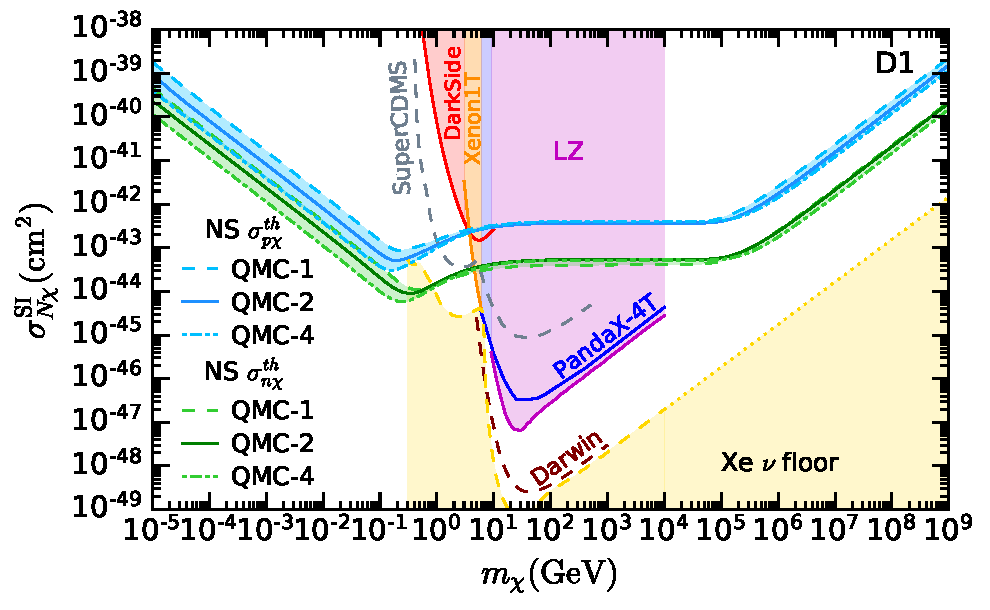
\includegraphics[width=0.6\textwidth]{capture_3/sigmath_mdm_SI_meff.pdf}
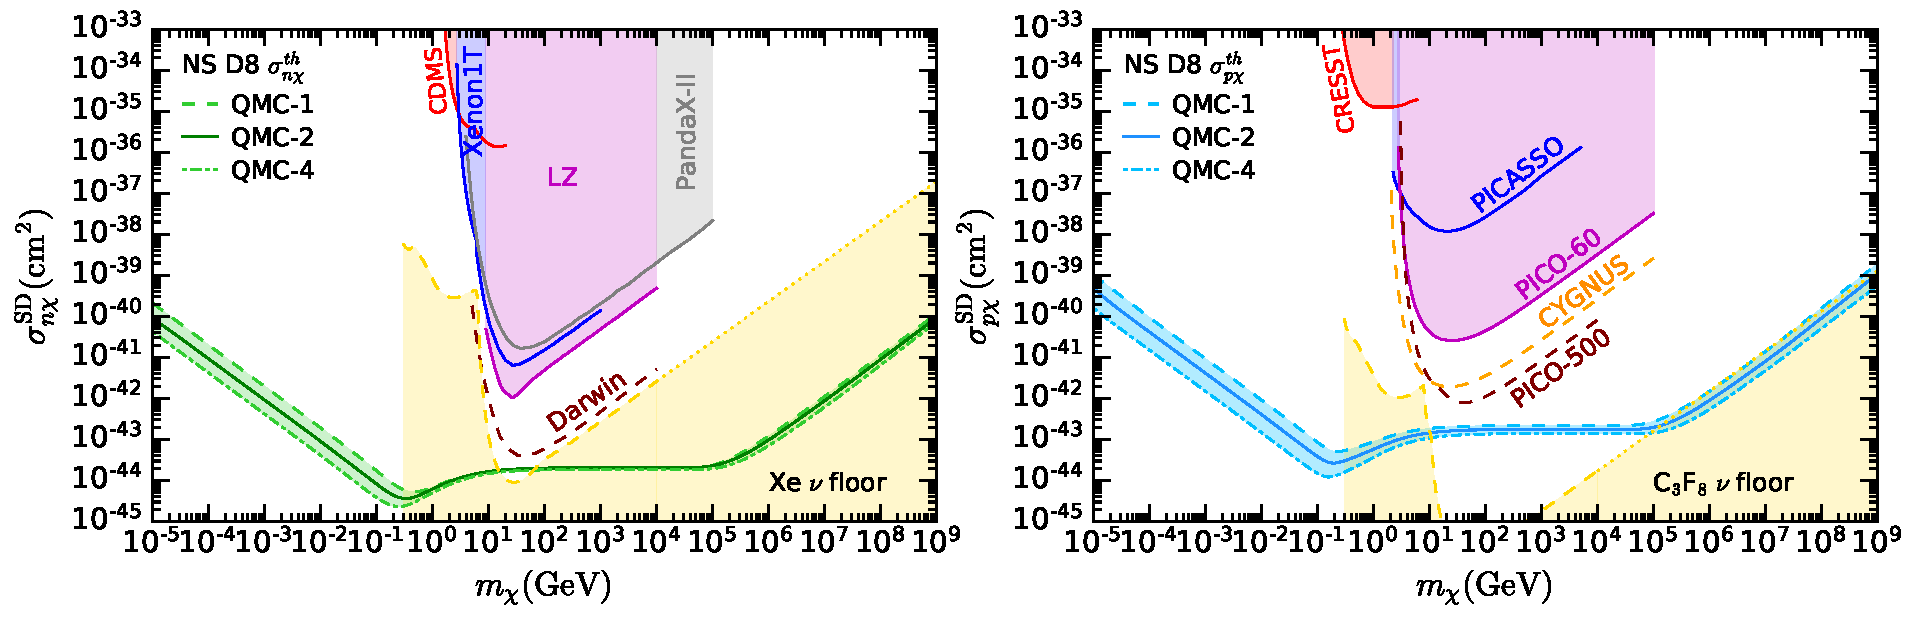
\includegraphics[width=\textwidth]{capture_3/sigmath_mdm_SD_meff.pdf}
   \caption{ DM-nucleon threshold cross-section for operators D1 (top) and D8 (bottom) for the QMC EoS family. The solid line represents $\sigmath$, computed assuming the NS configuration QMC-2. 
   We also show for comparison the leading spin-independent (SI) and spin-dependent (SD) DD limits from CDMSLite~\cite{SuperCDMS:2017nns_Lowmassdarkmatter}, DarkSide-50~\cite{DarkSide:2018bpj_Lowmassdarkmatter},  Xenon1T~\cite{XENON:2019rxp_ConstrainingspindependentWIMPnucleon,XENON:2019gfn_Lightdarkmatter, XENON:2019zpr_Searchlightdark,XENON:2020gfr_mar_SearchCoherentElastic}, PandaX-4T~\cite{PandaX-4T:2021bab_dec_DarkMatterSearch}, PICASSO~\cite{Behnke:2016lsk_apr_FinalResultsPICASSO} and PICO-60~\cite{PICO:2019vsc_jul_Darkmattersearch},  projected sensitivities from SuperCDMS SNOLAB Ge/Si~\cite{SuperCDMS:2016wui_ProjectedsensitivitySuperCDMS}, CDEX-1T~\cite{Yue:2016epq_CDEXdarkmatter}, CYGNUS  $10\m^3$~\cite{Vahsen:2020pzb_aug_CYGNUSFeasibilitynuclear},  PICO-500~\cite{VazquezJauregui_PICO500LSimulations500L} and Darwin~\cite{DARWIN:2016hyl_DARWINultimatedark}, as well as the neutrino coherent scattering background for xenon and $\mathrm{C_3F_8}$ bubble chamber detectors~\cite{Ruppin:2014bra_oct_Complementaritydarkmatter}.  
   } 
   \label{ch5:fig:sigmath}
\end{figure}
%%%%%%%%%%%%%%%%%%%%%%%%%%%%%%


For scalar-scalar spin-independent interactions (D1), the %XENON1T~\cite{Aprile:2018dbl} 
PandaX-4T~\cite{PandaX-4T:2021bab_dec_DarkMatterSearch} 
(magenta) direct detection experiment currently constrains cross-sections lower than $\sigmath$ in the $\sim10\GeV$ to $\sim10\TeV$ region.  In the rest of the parameter space, especially in the low mass region, the projected NS sensitivity surpasses any present or future DD experiment. In additon, NSs can rech sensitivities below the neutrino floor for a wide range of DM masses. In the case of spin-dependent interactions (D8) with either neutrons or protons, the projected NS sensitivity greatly surpasses the reach of all current and future DD experiments, for all DM masses. Moreover, for SD scattering off neutrons, the NS sensitivity is well below the neutrino floor for all DD targets in most of the parameter space. 


%%%%%%%%%%%%%%%%%%%%%%%%%%%%%%
%%%%%%%%%%%%%%%%%%%%%%%%%%%%%%
\section{Summary}
\label{ch5:sec:summary}
%%%%%%%%%%%%%%%%%%%%%%%%%%%%%%
%%%%%%%%%%%%%%%%%%%%%%%%%%%%%%

We have extended the framework for dark matter capture in neutron stars to account for the effect of hadronic structure, through the use of momentum-dependent form factors, and to incorporate baryon interactions in the degenerate NS medium, rather than modeling the baryons as a free Fermi gas. 

Incorporating these effects into the formalism presented in Chapter~\ref{chapter:capture_intro}, we find a reduction in the rate at which DM is captured by scattering on nucleons.  The consequences of this is that the threshold cross-section is increased by at least $\sim$ one order of magnitude for $m_\chi\gtrsim10\GeV$. The exact size of the effect depends on the NS configuration and the type of DM-nucleon interaction, being stronger for scalar and pseudoscalar EFT operators. Interestingly, incorporating these effects reduces the variation of the threshold cross-section associated with different choices for the NS equation of state.

For proton targets, the use of the interacting baryon approach to obtain the correct Fermi energy is particularly important.  The standard free Fermi gas approach leads to the incorrect conclusion that protons are non-degenerate in the outer regions of the core, and hence not subject to Pauli blocking, greatly enhancing the capture rate due to DM-proton scattering, even surpassing that due to DM-neutron scattering.  However, with the use of the correct Fermi energy, obtained by incorporating nucleon-strong interactions via effective masses, the Pauli suppression of the proton final states is recovered. 

Heavy NSs may also contain exotic matter in the form of hyperons within the innermost regions of the NS core. We have found that scattering of DM with hyperons can enhance the DM capture rate in the case of pseudoscalar DM-baryon interactions, with the hyperon contribution at least comparable to that of neutrons over the entire DM mass range.

Finally, we note that, despite somewhat reduced capture rates compared to the standard treatment in the literature, the projected NS sensitivity remains much greater than that for direct detection experiments for both the spin-independent scattering of light (sub-GeV) DM, or for the spin-dependent scattering of DM of any mass.  
